\documentclass[11pt]{article}

\oddsidemargin=17pt \evensidemargin=17pt
\headheight=9pt     \topmargin=26pt
\textheight=564pt   \textwidth=433.8pt
\date{}
\usepackage{url}
\usepackage{amsmath}
\usepackage{amsfonts,amssymb,amsthm,cite,float,graphicx}
\usepackage{physics}
\usepackage{graphicx}
\usepackage{mathtools}
\usepackage{float}
\usepackage{hyperref}

%new math symbols taking no arguments
\newcommand\0{\mathbf{0}}
\newcommand\CC{\mathbb{C}}
\newcommand\FF{\mathbb{F}}
\newcommand\NN{\mathbb{N}}
\newcommand\QQ{\mathbb{Q}}
\newcommand\RR{\mathbb{R}}
\newcommand\ZZ{\mathbb{Z}}
\newcommand\bb{\mathbf{b}}
\newcommand\kk{\Bbbk}
\newcommand\mm{\mathfrak{m}}
\newcommand\pp{\mathfrak{p}}
\newcommand\xx{\mathbf{x}}
\newcommand\yy{\mathbf{y}}
\newcommand\GL{\mathit{GL}}
\newcommand\into{\hookrightarrow}
\newcommand\nsub{\trianglelefteq}
\newcommand\onto{\twoheadrightarrow}
\newcommand\minus{\smallsetminus}
\newcommand\goesto{\rightsquigarrow}
\newcommand\nsubneq{\vartriangleleft}

%redefined math symbols taking no arguments
\newcommand\<{\langle}
\renewcommand\>{\rangle}
\renewcommand\iff{\Leftrightarrow}
\renewcommand\phi{\varphi}
\renewcommand\implies{\Rightarrow}

%new math symbols taking arguments
\newcommand\ol[1]{{\overline{#1}}}

%redefined math symbols taking arguments
\renewcommand\mod[1]{\ (\mathrm{mod}\ #1)}

%roman font math operators
\DeclareMathOperator\aut{Aut}

%for easy 2 x 2 matrices
\newcommand\twobytwo[1]{\left[\begin{array}{@{}cc@{}}#1\end{array}\right]}

%for easy column vectors of size 2
\newcommand\tworow[1]{\left[\begin{array}{@{}c@{}}#1\end{array}\right]}

\newtheorem{theorem}{Theorem}
\newtheorem{corollary}{Corollary}[theorem]
\newtheorem{lemma}[theorem]{Lemma}
\newtheorem{exercise}[theorem]{Exercise}
\newtheorem{definition}[theorem]{Definition}

\title{Quantum Algorithms and Learning Theory\\\textit{Notes and Exercises}}
\author{Faris Sbahi}

\begin{document}
\maketitle

\tableofcontents

\section{Nielsen \& Chuang: Chapter 2}

\begin{exercise} (2.11) Find the eigenvectors and eigenvalues of the Pauli matrices. 

\begin{proof}
	\begin{align*}
	X &= \begin{bmatrix}
 0 & 1 \\ 1 & 0	
 \end{bmatrix} \\
 X - \lambda I &= \begin{bmatrix}
 -\lambda & 1 \\ 1 & -\lambda	
 \end{bmatrix} \\
 \lambda^2 - 1 &= 0 \\
 \lambda_{\pm} &= \pm 1 \\
 \begin{bmatrix}
 -1 & 1 \\ 1 & -1
 \end{bmatrix} v_+ &= 0 \\
 \implies v_+ = \frac{1}{\sqrt{2}}\begin{bmatrix}
 1 \\ 1
 \end{bmatrix} \\
 \begin{bmatrix}
 1 & 1 \\ 1 & 1
 \end{bmatrix} v_- &= 0 \\
 \implies v_- = \frac{1}{\sqrt{2}}\begin{bmatrix}
 1 \\ -1
 \end{bmatrix}
	\end{align*}

Similarly, $Y$ has eigenvalues $\pm 1$ with respective eigenvectors $\Big\{ \begin{bmatrix}
 1 \\ i
 \end{bmatrix} , \begin{bmatrix}
 1 \\ -i
 \end{bmatrix} \Big\}$. $Z$ has eigenvalues $\pm 1$ with respective eigenvectors $\Big\{ \begin{bmatrix}
 1 \\ 0
 \end{bmatrix} , \begin{bmatrix}
 0 \\ 1
 \end{bmatrix} \Big\}$
\end{proof}
	
\end{exercise}

\subsection{Postulates of Quantum Mechanics}

First, we cover the fundamental postulates of quantum mechanics. 

\subsubsection{State Space and State Vector}

Associated with an isolated physical system is a Hilbert space, $\mathcal{H}$. A Hilbert space is a complete inner-product vector space. Note that completeness holds trivially in a finite-dimensional vector space because we have closure with respect to all sequences (and hence any Cauchy sequence in the vector space must converge to a vector in the same space). Nevertheless, the state space of a physical system may be infinite-dimensional. 

A system is completely described by a unit vector $u \in \mathcal{H}$ called the state vector.

For example, consider a system given by a single qubit, which has a two-dimensional state space. Let $\ket{0}$ and $\ket{1}$ be an orthonormal basis for this space. Hence, a state vector in this space is given by 

\begin{align*}
\ket{\psi} = a\ket{0} + b\ket{1}	
\end{align*}


where $a, b \in \CC$ and $|a|^2 + |b|^2 = 1$. 

\subsubsection{Evolution}\label{post-discrete-evol}

The evolution of a closed quantum system is described by a unitary transformation. Recall that an operator $U$ is unitary iff $U^\dagger U = I = UU^\dagger$ (and hence preserves inner products\footnote{and furthermore has a spectral decomposition because it is normal}).

So, let the state of a system at time $t_1$ be given by $\ket{\psi}$ and $\ket{\psi'}$ at $t_2$. Hence,

\begin{align*}
\ket{\psi'} = U\ket{\psi}	
\end{align*}

\begin{exercise}
(2.51) Verify that $H$ is unitary 

\begin{align*}
HH^\dag &= 1/2\begin{pmatrix} 1 & 1 \\ 1 & -1\end{pmatrix}\begin{pmatrix} 1 & 1 \\ 1 & -1\end{pmatrix} \\
&= 1/2\begin{pmatrix} 2 & 0 \\ 0 & 2 \end{pmatrix} \\
&= I = H^\dag H
\end{align*}
\end{exercise}

\begin{exercise}
(2.52) Verify that $H^2 = I$

Because $H$ is hermitian we have that 

\begin{align*}
H^2 &= HH^\dag \\
&= I
\end{align*}

from $H$ being unitary.
\end{exercise}

\begin{exercise}
(2.53) What are the eigenvalues and eigenvectors of $H$?

\begin{align*}
\det \frac{1}{\sqrt{2}}\begin{pmatrix} 1 - \lambda & 1 \\ 1 & -1 - \lambda\end{pmatrix}
&= -(1-\sqrt{2}\lambda)(1+\sqrt{2}\lambda) - 1 = 0 \\
&= -1 + 2\lambda^2 -1 \\
\lambda &= \pm 1 \\
\frac{1}{\sqrt{2}}\begin{pmatrix} 1-\sqrt{2} & 1 \\ 1 & -1 +\sqrt{2}\end{pmatrix}v_1 &= 0 \\
(1-\sqrt{2})v_{11} + v_{12} &= 0 \\
v_{11} -(1-\sqrt{2})v_{12} &= 0 \\
v_1 &= \begin{pmatrix} 1 + \sqrt{2} \\ 1\end{pmatrix} \\
\frac{1}{\sqrt{2}}\begin{pmatrix} 1+\sqrt{2} & 1 \\ 1 & -1 -\sqrt{2}\end{pmatrix}v_2 &= 0 \\ 
v_2 &= \begin{pmatrix} 1 - \sqrt{2} \\ 1\end{pmatrix}
\end{align*}
	
\end{exercise}

\subsubsection{Evolution in Continuous Time}\label{post-cts-evol}

Schrodinger's equation provides the time evolution of the state of a quantum system

\begin{align}\label{schro-cts}
i\hbar \frac{d\ket{\psi}}{dt} = H\ket{\psi}	
\end{align}

where $H$ is the (Hermitian) Hamiltonian of the closed system. Because the Hamiltonian is Hermitian it has spectral decomposition 

\begin{align*}
H = \sum_{E} E \ket{E}\bra{E}	
\end{align*}

where $E$ is the energy eigenvalue corresponding to energy eigenstate $\ket{E}$. 

For example, consider the Hamiltonian $H = \hbar \omega X$  (recall that $X = \sigma_X = \begin{pmatrix} 0 & 1 \\ 1 & 0\end{pmatrix}$ from \ref{pauli}). Hence, we solve for its eigenvalues and eigenvectors

\begin{align*}
	\det{ \hbar\omega\begin{pmatrix} -\lambda & 1 \\ 1 & -\lambda\end{pmatrix}} &= 0 \\
	\lambda^2 - 1^2 &= 0 \\
	\lambda &= \pm 1 \\
	\implies E_{\pm} &= \pm \hbar \omega \\
	\hbar\omega\begin{pmatrix} -1 & 1 \\ 1 & -1\end{pmatrix}\ket{E_+} &= 0 \\
	\ket{E_+} &= \frac{1}{\sqrt{2}}\begin{pmatrix}
		1 \\ 1
	\end{pmatrix} \coloneqq \ket{+} \\
	\ket{E_-} &= \ket{-}
\end{align*}

Onwards, notice that we can solve Schrodinger's equation (\ref{schro-cts}) and have

\begin{align*}
	\ket{\psi(t_2)} &= \exp[\frac{-iH(t_2 - t_1)}{\hbar}] \ket{\psi(t_1)}
\end{align*}

and equivalently from \ref{post-discrete-evol} we can represent this transformation with unitary operator $U = \exp[\frac{-iH(t_2 - t_1)}{\hbar}]$. This holds in general and so we can consider the two descriptions from \ref{post-discrete-evol} and \ref{post-cts-evol} interchangeably (the authors prefer the latter). 

\begin{exercise}
(2.54) Suppose $[A, B] = 0$ and $A, B$ are Hermitian. Prove that $\exp(A)\exp(B) = \exp(A + B)$

\begin{proof}
	From Theorem 2.2, $A$ and $B$ are simultaneously diagonalizable. Hence, there is a common set of orthonormal eigenvectors $\{ \ket{i} \}$. Hence,
	
	$A = \sum_i a_i \ket{i}\bra{i}, B = \sum_i b_i \ket{i}\bra{i}$. So, 
	
	\begin{align*}
	\exp(A)\exp(B) &= \sum_{k'=0}^\infty\sum_{i'} \frac{(b_{i'} \ket{i'}\bra{i'})^{k'}}{k'!}\sum_{k=0}^\infty\sum_{i} \frac{(a_i \ket{i}\bra{i})^k}{k!} \\
	\intertext{By orthonormality,}
	&= \sum_{i}\Big[\sum_{k'=0}^\infty \frac{b_i^{k'} \ket{i}\bra{i}}{k'!}\sum_{k=0}^\infty \frac{a_i^k \ket{i}\bra{i}}{k!}\Big] \\
	&= \sum_{i}\sum_{k'=0}^\infty\sum_{k=0}^\infty \frac{a_i^k b_i^{k'} \ket{i}\bra{i}}{k!k'!}\\
	&= \sum_{i}\sum_{l=0}^\infty\sum_{k=0}^l \frac{a_i^k b_i^{l-k} \ket{i}\bra{i}}{k!(l-k)!}\\
	&= \sum_{i}\sum_{l=0}^\infty \frac{1}{l!}\sum_{k=0}^l \binom{k}{l} a_i^k b_i^{l-k} \ket{i}\bra{i} \\
	&= \sum_{i}\sum_{l=0}^\infty \frac{(a_i +b_i)^l}{l!} \ket{i}\bra{i} \\
	&= \exp(A + B)
	\end{align*}
\end{proof}
\end{exercise}

\begin{exercise}
(2.55) Prove that $U(t_1, t_2)$ is unitary	
\begin{proof}

Using the result of 2.54, 
	\begin{align*}
	UU^\dag = U^\dag U &= \exp[\frac{-iH(t_2 - t_1)}{\hbar}]\exp[\frac{iH(t_2 - t_1)}{\hbar}] \\
	&= 	\exp(\hat{0}) \\
	&= 	I
	\end{align*}
\end{proof}
\end{exercise}

\begin{exercise}
(2.56) Use the spectral decomposition to show that $K \coloneqq -i\log U$ is Hermitian for any unitary $U$ and thus $U = \exp(iK)$ for some Hermitian $K$
\begin{proof}
	The eigenvalues of $U$ can be given as $\exp(i\theta)$ by unitary. Furthermore, from spectral theorem, $U$ is diagonalizable as $U = V \Lambda V^\dag$ where $V$ is unitary\footnote{Quick proof: $U$ can be written as $U=VTV^\dag$ where $V$ is unitary and $T$ is upper triangular by Schur Decomposition. However, $UU^\dag = U^\dag U, VV^\dag = I = V^\dag V$ $\implies$ $T$ is normal $\implies$ $T$ is diagonal.}. Hence, $U = V \Lambda V^\dag$ where diagonal matrix $\Lambda$ has elements of the form $\exp(i\theta)$ across the diagonal. 
	
	Furthermore, $(V\Lambda V^\dag)^n = V\Lambda V^\dag V\Lambda V^\dag\cdots V\Lambda V^\dag = V\Lambda^n V^\dag$ $\implies$ $\exp(V \Lambda V^\dag) = V \exp(\Lambda) V^\dag$. Therefore, let $\Lambda' = \log(\Lambda)$ which therefore has elements of the form $i\theta$. Hence, $U = \exp(V \Lambda' V^\dag)$ 
	
	\begin{align*}
		K &= -i\log U \\
		&= -i\log (\exp(V \Lambda' V^\dag)) \\
		&= -iV \Lambda' V^\dag \\
		&= V\Theta V^\dag
	\end{align*}

where $\Theta = -i\Lambda'$ has elements of the form $\theta$ (and hence the elements are real along the diagonal and zero elsewhere $\implies$ $\Theta^\dag = \Theta$). Therefore, $K^\dag = V^\dag\Theta^\dag V = V\Theta V^\dag = K$.
\end{proof}
\end{exercise}

\subsubsection{Quantum Measurement}\label{qmeas}

Quantum measurements are described by a collection of measurements operators $\{ M_m \}$ (where the index $m$ refers to the potential measurement outcomes of the experiment) which act on the state space of the system being observed. 

Hence, if the pre-measurement state is $\ket{\psi}$, then 

\begin{align*}
	p(m) = \bra{\psi} M_m^\dagger M_m \ket{\psi}
\end{align*}

and the post-measurement state is 

\begin{align*}
	\frac{M_m \ket{\psi}}{\sqrt{p(m)}}
\end{align*}

Furthermore, $\{ M_m \}$ satisfy the completeness equation

\begin{align*}
\sum_m M_m^\dagger M_m = I
\end{align*}

An important example of a measurement is the measurement of a qubit in the computational basis. This is a measurement of a qubit with two outcomes defined by the measurement operators $M_0 = \ket{0}\bra{0}$ and $M_1 = \ket{1}\bra{1}$.

Now, we see an interesting implication. If we seek to distinguish our physical system from a set of orthogonal states, then we can reliably do so by simply defining each measurement operator to be the outer product of our states of interest. We add a final operator defined to be the remaining complement of the identity in order to satisfy the completeness equation. 

On the flipside, two non-orthogonal states $\ket{\psi_1}$ and $\ket{\psi_2}$ necessarily share a parallel component in their orthogonal decomposition. Hence, a measurement outcome that corresponds to the pre-measurement state being $\ket{\psi_1}$ with probability $p = 1$ has a probability $p'>0$ of having been in state $\ket{\psi_2}$. 

\begin{exercise}
(2.57) Suppose $\{L_l\}$ and $\{M_m\}$ are two sets of measurement operators. Show that a measurement defined by the measurement operators $\{L_l \}$ followed by a measurement defined by the measurement operators $\{ M_m \}$ is physically equivalent to a single measurement defined by measurement operators $\{N_{lm}\}$ with the representation $N_{lm} = M_mL_l$.
\begin{proof}
Let $\ket{\phi}$ be our initial state and recall that if $l$ is measured then the post-measurement state is given by $\frac{L_l \ket{\psi}}{\sqrt{p(l)}}$. Furthermore, if we then measure $m$ we have 	$\frac{M_m(L_l \ket{\psi})}{\sqrt{p(m)}\sqrt{p(l)}} = \frac{N_{lm} \ket{\psi})}{\sqrt{p(m)p(l)}}$. 

Now, 

\begin{align*}
p(m)p(l) &= \bra{\psi} L_l^\dagger L_l \ket{\psi}\frac{\bra{\psi} L_l^\dagger}{\sqrt{p(m)}}M_m^\dag M_m \frac{L_l \ket{\psi}}{\sqrt{p(m)}} \\
&= p(l) \frac{\bra{\psi} L_l^\dagger M_m^\dag M_m L_l \ket{\psi}}{p(l)}\\
&= \bra{\psi} N_{lm}^\dagger N_{lm} \ket{\psi}\\
&= p(lm)
\end{align*}

Hence, $\frac{N_{lm} \ket{\psi}}{\sqrt{p(m)p(l)}}=\frac{N_{lm} \ket{\psi}}{\sqrt{p(lm)}}$. Therefore, the representation is physically equivalent.
\end{proof}

\end{exercise}

\subsubsection{Projective Measurements}

There exists a special class of quantum measurements known as projective measurements. These measurements can be described by an observable $M$, a hermitian operator on the state space being observed. $M$ has spectral decomposition

\begin{align*}
M = \sum_m m P_m	
\end{align*}

where $P_m$ is the projector onto the eigenspace of $M$ with eigenvalues $m$. 

Furthermore, if the pre-measurement state is $\ket{\psi}$, then 

\begin{align*}
p(m) = 	\bra{\psi} P_m \ket{\psi}
\end{align*}

and the post-measurement state is 

\begin{align*}
	\frac{P_m \ket{\psi}}{\sqrt{p(m)}}
\end{align*}

This simplifies the formula for the expected value of a measurement

\begin{align*}
\langle M \rangle &= \sum_m m p(m) \\
&= \bra{\psi} (\sum_m m P_m)  \ket{\psi} \\
&= 	\bra{\psi} M \ket{\psi}
\end{align*}

\begin{exercise}
	(2.58) Suppose we prepare a quantum system in an eigenstate $\ket{\psi}$ of some observable $M$, with corresponding eigenvalue $m$. What is the average observed value of $m$ and the standard deviation?
	
	\begin{proof}
		First, 
		
		\begin{align*}
	\< M \> &= \bra{\psi} M 	\ket{\psi} \\
	&= \bra{\psi} m \ket{\psi} = m
	\end{align*}
	
	Furthermore,

	\begin{align*}
	\< M^2 \> - \< M \>^2 &= \bra{\psi} M^2 	\ket{\psi} - m^2 \\
	&= \bra{\psi} M^\dag M \ket{\psi} -m^2 \\
	&= m^2 - m^2 = 0
	\end{align*}
	\end{proof}	
	
\end{exercise} 

For example, consider projective measurements on the system given by single qubits with observable Pauli matrix $Z$. Hence, $Z$ has eigenvalues $+1$ and $-1$ and eigenstates $\ket{0}$ and $\ket{1}$, respectively. So, consider state $\ket{\psi} = \frac{\ket{0} + \ket{1}}{\sqrt{2}}= \ket{+}$ $\implies$ $p(+1) = \bra{+}\ket{0}\bra{0}\ket{+} = \frac{1}{2}$. Similarly, $p(-1) = \frac{1}{2}$. 

More generally, suppose $v$ is an arbitrary 3-d vector. We can define an observable

\begin{align*}
v \cdot \sigma = v_1\sigma_x + v_2 \sigma_y + v_3\sigma_z
\end{align*}

\begin{exercise}
	(2.59) Suppose we have a qubit in the state $\ket{0}$, and we measure the observable $X$. What is the average value of $X$? What is the standard deviation of $X$?
	
	\begin{proof}
		$X$ has eigenvalues $+1$ and $-1$ and eigenstates $\ket{+}$ and $\ket{-}$, respectively. Hence,
		
	\begin{align*}
	\< X \> &= \bra{\psi} X 	\ket{\psi} \\
	&= \bra{\psi} (\ket{+}\bra{+} - \ket{-}\bra{-}) \ket{\psi} \\
	&= \bra{0}\ket{+}\bra{+}\ket{0} - \bra{0}\ket{-}\bra{-}\ket{0}\\
	&= \frac{1}{2} - \frac{1}{2} = 0
	\end{align*}
	
	Furthermore,

	\begin{align*}
	\< M^2 \> - \< M \>^2 &= \bra{\psi} M^2 	\ket{\psi} - 0 \\
	&= \bra{\psi} (\ket{+}\bra{+} + \ket{-}\bra{-}) \ket{\psi} \\
	&= \frac{1}{2} + \frac{1}{2} = 1
	\end{align*}
	\end{proof}
	
\end{exercise}

\begin{exercise}
	(2.60) Show that $v \cdot \sigma$ has eigenvalues $\pm 1$ and that the projectors onto the corresponding eigenspaces are given by $P_{\pm} = (I \pm v \cdot \sigma)/2$.

\begin{proof}
	First, $v\cdot \sigma$ is Hermitian so it's spectral decomposition is given by $v \cdot \sigma = U \Lambda U^\dag$ for some unitary $U$, diagonal matrix $\Lambda$. Hence, using $(v\cdot \sigma)^2 = I$ we have
	
	\begin{align*}
		I &= (v \cdot \sigma)^2 = (U \Lambda U^\dag)^2 \\
		&= U \Lambda^2 U^\dag \\
		\implies U^\dag I U &= \Lambda^2 \\
		I & = \Lambda^2
	\end{align*}

Therefore, $\Lambda$ must have diagonal entries $\pm 1$. 

Next, $P_i P_j = \delta_{ij}P_j$ since if $i \neq j$ then $(I + v \cdot \sigma)(I - v\cdot \sigma) = I - (v \cdot \sigma)^2 = I - I = 0$. Furthermore, $P_+ + P_- = (I + v \cdot \sigma)/2 + (I - v \cdot \sigma)/2 = I$. 

Finally, $(+1)P_+ + (-1)P_- = (I + v \cdot \sigma)/2 - (I - v \cdot \sigma)/2 = v \cdot \sigma$. 
\end{proof}
\end{exercise}

\begin{exercise}
	(2.61) Calculate the probability of obtaining result $+1$ for a measurement of $v \cdot \sigma$, given that the state prior to measurement is $\ket{0}$. What is the state of the system after measurement if $+1$ is obtained?
	
	\begin{proof}
	
	First, 
	
		\begin{align*}
			p(+1) &= \bra{\psi} P_+ \ket{\psi} \\
			&= \bra{\psi}(I + v \cdot \sigma)/2\ket{\psi} \\
			&= 1 + \frac{1}{2}[ v_1\bra{0} X \ket{0} + v_2\bra{0} Y \ket{0} + v_3\bra{0} Z \ket{0}] \\
			&= 1 + \frac{1}{2}[ v_1\bra{0}\ket{1} + iv_2\bra{0}\ket{1} + v_3\bra{0}\ket{0}] \\
			&= 1+ \frac{v_3}{2}
		\end{align*}
	
	Furthermore, after measurement of $+1$ we have
	
	\begin{align*}
		(I + v \cdot \sigma)/2\ket{0} &= \ket{0} + \frac{1}{2}[ v_1\ket{1} + iv_2\ket{1} + v_3\ket{0}] \\
		&= \Big[\big(\frac{v_3}{2} + 1\big)\ket{0} + \frac{v_1 + iv_2}{2}\ket{1}\Big]/\sqrt{1+ \frac{v_3}{2}}
	\end{align*}

	\end{proof}
\end{exercise}

\subsubsection{POVM measurements}\label{povm}

POVMs are best viewed as a special case of the general measurement formalism, providing the simplest means to study post-measurement statistics without knowledge of the post measurement state.

From above, $p(m) = \bra{\psi} M_m^\dagger M_m \ket{\psi}$ so if we define $E_m \coloneqq M_m^\dagger M_m$ (which is hence positive from \ref{posop}) then these $E_m$'s are sufficient for the purpose of computing probabilities. We denote $\{ E_m \}$ as a POVM. POVMs also satisfy the completeness relation.

Note that projective operators are the special case of being equivalent to their respective POVM element because $E_m = P_m^\dag P_m = P_m$. 

\begin{exercise}
(2.62) Show that any measurement where the measurement operators and the POVM elements coincide is a projective measurement

\begin{proof}
We would then have $M_m = E_m = M_m^\dag M_m$. Furthermore, $E_m$ is a positive operator $\implies$ $M_m = M_m^\dag M_m = M_m M_m^\dag = M_m^\dag$ so $M_m$ is Hermitian. Hence, $M_m = M_m^2$ so the measurement is projective.
\end{proof}	
\end{exercise}

Nevertheless, the POVM formalism is a useful guide in for our intuition in quantum information. Consider if Alice prepares some state for Bob that is either $\ket{\psi_1} = \ket{0}$ or $\ket{\psi_2} = \frac{\ket{0} + \ket{1}}{\sqrt{2}}$. Recall from \ref{qmeas}, Bob can't determine which state was prepared with full certainty (because of the shared orthogonal component $\ket{0}$). Still, we can define a POVM\footnote{verify that completeness and these being positive operators holds}

\begin{align*}
E_1 &= \frac{\sqrt{2}}{1+\sqrt{2}}\ket{1}\bra{1}	\\
E_2 &= \frac{\sqrt{2}}{1+\sqrt{2}}\frac{(\ket{0} - \ket{1})(\bra{0} - \bra{1})}{2} \\
E_3 &= I - E_1 - E_2
\end{align*}

Now, notice what happens. 

\begin{align*}
\bra{\psi_1} E_1 \ket{\psi_1} &= \bra{0} \frac{\sqrt{2}}{1+\sqrt{2}}\ket{1}\bra{1}\ket{0} \\
	&= 0 \\
\bra{\psi_2} E_1 \ket{\psi_2} &= \frac{\bra{0} + \bra{1}}{\sqrt{2}}\frac{\sqrt{2}}{1+\sqrt{2}}\ket{1}\bra{1}\frac{\ket{0} + \ket{1}}{\sqrt{2}} \\
	&= \frac{\sqrt{2}}{2\sqrt{2} + 2} > 0 
\end{align*}

Hence, if we observe $E_1$ after the measurement described by $\{ E_1, E_2, E_3 \}$, then Alice must've prepared $\ket{\psi_2}$. Similarly,

\begin{align*}
\bra{\psi_1} E_2 \ket{\psi_1} &= \bra{0} \frac{\sqrt{2}}{1+\sqrt{2}}\frac{(\ket{0} - \ket{1})(\bra{0} - \bra{1})}{2}\ket{0} \\
	&= \frac{\sqrt{2}}{2\sqrt{2} + 2} > 0 \\
\bra{\psi_2} E_2 \ket{\psi_2} &= \frac{\bra{0} + \bra{1}}{\sqrt{2}}\frac{\sqrt{2}}{1+\sqrt{2}}\frac{(\ket{0} - \ket{1})(\bra{0} - \bra{1})}{2}\frac{\ket{0} + \ket{1}}{\sqrt{2}} \\
	&= 0
\end{align*}

so if we observe $E_2$, then Bob concludes that Alice prepared $\ket{\psi_1}$. Our routine is imperfect because we may observe $E_3$ and hence would infer nothing of the original state. Still, we would never $\textit{incorrectly}$ guess given that we allow ourselves to abstain when we see $E_3$. 

\begin{exercise} (2.63) Suppose a measurement is described by measurement operators $M_m$. Show that there exist unitary operators $U_m$ such that $M_m  = U_m\sqrt{E_m}$ where $E_m$ is the POVM associated to the measurement. 

\begin{proof}
From SVD, we have that $M_m = UDV$ for $U,V$ unitary and $D$ real, diagonal. Hence,

\begin{align*}
\sqrt{E_m} &= \sqrt{M_m^\dag M_m} = \sqrt{V^\dag DU^\dag UDV} \\ 	
&= \sqrt{V^\dag D^2V} \\
&= V^\dag DV = V^\dag U^\dag UDV \\
&= U_m^\dag M_m
\end{align*}
 
where $U_m \coloneqq UV$. Therefore, there exists the unitary transformation of interest.

\end{proof}
\end{exercise}

\begin{exercise} (2.64) Suppose Bob is given a quantum state chosen from a set $S = \ket{\psi_1} , \cdots , \ket{\psi_m}$ of linearly independent states. Construct a POVM $\{ E_1 , \cdots , E_{m+1} \}$ such that if outcome $E_i$ occurs, $1 \leq i \leq m$, then Bob knows with certainty that he was given state $\ket{\psi_i}$.

\begin{proof}
	To distinguish the states we require $\bra{\psi_i} E_j \ket{\psi_i} = p_i \delta_{ij}$ where $p_i > 0$ and $1 \leq i,j \leq m$. 

So, we can use the Gram-Schmidt process using $S$ as our linearly independent set. This will give us an orthonormal set $U = \ket{\phi_1} , \cdots , \ket{\phi_m}$ that spans the same subspace as $S$. Next, we can represent each $\ket{\psi_i}$ in this orthonormal basis, $U$. Finally, for each $i$ we can find a vector $\ket{\psi'_i}$ in the span of $U$ that is orthogonal to all $\ket{\psi_j}, j \neq i$. Hence, we can define $E_i = \ket{\psi_i'} \bra{\psi_i'}, 1 \leq i \leq m$. Finally, take $E_{m+1} = I - \sum_m E_i$. 

Creating an optimal POVM is much trickier (in the sense of minimizing the probability $p_{m+1}$).
\end{proof}
\end{exercise}

From this exercise, we see that POVMs present a reliable way to distinguish non-orthogonal (but linearly independent) states given that we allow for the slack of an "inconclusive" measurement ($E_{m+1}$). 

\begin{exercise} (2.65) Express the states $(\ket{0} + \ket{1})/\sqrt{2}$ and $(\ket{0} - \ket{1})/\sqrt{2}$ in a basis in which they are not the same up to relative phase shift.

\begin{proof}
Trivially, the $\ket{+}$ and $\ket{-}$ suffices as a basis where they are not the same up to relative phase shift.	
\end{proof}

	
\end{exercise}

\subsubsection{Composite Systems}

The state space of a composite physical system is the tensor product of the state spaces of the component physical systems. 

\begin{exercise} (2.66)
	Show that the average value of the observable $X_1Z_2$ ($X$ acting on the first qubit and $Z$ on the second) for a two qubit system measured in the state $\frac{\ket{00} + \ket{11}}{\sqrt{2}}$ is zero.
\end{exercise}

\begin{proof}
	Let observable $M = X_1Z_2$. Hence, 
	
	\begin{align*}
	\langle M \rangle &= \frac{\bra{00} + \bra{11}}{\sqrt{2}} M \frac{\ket{00} + \ket{11}}{\sqrt{2}}\\	
	&= \frac{\bra{00} + \bra{11}}{\sqrt{2}}\frac{X_1\ket{0}Z_2\ket{0} + X_1\ket{1}Z_2\ket{1}}{\sqrt{2}} \\
	&= \frac{\bra{00} + \bra{11}}{\sqrt{2}}\frac{\ket{1}\ket{0} - \ket{0}\ket{1}}{\sqrt{2}} \\
	&= 0
	\end{align*}
\end{proof}
 
Interestingly, we can show that a general quantum measurement (as described in \ref{qmeas}) can be implemented as a projective measurement coupled with unitary dynamics.

Consider a quantum system with state space $Q$ and measurements $M_m$ on this system. We can introduce an \textit{ancilla} system $M$ with orthonormal basis $\ket{m}$ which is in one-to-one correspondence with the possible outcomes of the measurement we wish to implement. 

So, let $\ket{0}$ be a fixed state of $M$ and define an operator $U$ on $\ket{\psi}\ket{0}$ (with $\ket{\psi}$ as a state of $Q$) by

\begin{align*}
U\ket{\psi}\ket{0} \coloneqq \sum_m M_m \ket{\psi}\ket{m}
\end{align*}

Hence,

\begin{align*}
\bra{\phi}\bra{0}U^\dag U \ket{\psi}	 \ket{0} &= \sum_m \sum_{m'} \bra{\phi} M_m^\dag M_{m'} \ket{\psi}\bra{m}\ket{m'} \\
\intertext{So, because the states $\ket{m}$ are orthonormal}
&= \sum_m\bra{\phi} M_m^\dag M_{m} \ket{\psi} \\
\intertext{and finally by the completeness of $M_m$}
&= \bra{\phi}\ket{\psi}
\end{align*}

This tells us that $U$ preserves inner products between states of the form $\ket{\psi}\ket{0}$. Furthermore, we can show that $U$ can be extended to a unitary operator on $Q \otimes M$ (exercise).

\begin{exercise}
(2.67)
% TODO 2.67
\end{exercise}

Hence, consider a projective measurement on the two systems ($U\ket{\psi}\ket{0}$) given by projectors $P_m \coloneqq I_Q \otimes \ket{m}\bra{m}$. So,

\begin{align*}
p(m) &= \bra{\psi} \bra{0} U^\dag P_m U \ket{\psi} \ket{0} \\
&= \sum_{m'}\sum_{m''} \bra{\psi} M_{m'}^\dag \bra{m'} (I_Q \otimes \ket{m}\bra{m})M_{m''} \ket{\psi} \ket{m''} \\
&= \bra{\psi} M_m^\dag M_m \ket{\psi}
\end{align*}

which agrees with the general result from \ref{qmeas}. Similarly, the post-measurement state is as expected. Hence, we've shown that unitary dynamics, projective measurements, and ancillary systems can be used together to describe any general measurement.

\begin{exercise}
(2.68) Prove that $\ket{\psi} \neq \ket{a}\ket{b}$ for all single qubit state $\ket{a}$ and $\ket{b}$ where $\ket{\psi} = \frac{\ket{00} + \ket{11}}{\sqrt{2}}$.
\end{exercise}

\begin{proof}
	First, decompose the qubit state in their basis, $\ket{a} = \alpha_0 \ket{0} + \alpha_1 \ket{1}$ and $\ket{b} = \beta_0 \ket{0} + \beta_1 \ket{1}$. Now, we prove by contradiction
	
	\begin{align*}
	\ket{a}\ket{b} &= \alpha_0\beta_0 \ket{00} + \alpha_0\beta_1 \ket{01} + \alpha_1\beta_0 \ket{10} + \alpha_1\beta_1 \ket{11} \\
	&= \frac{\ket{00} + \ket{11}}{\sqrt{2}}
	\end{align*}

which would imply that either $\alpha_0$ or $\beta_1$ are zero in order to remove the $\ket{01}$ term. However, this would also remove either the $\ket{00}$ or $\ket{11}$ term, so we have a contradiction.
\end{proof}

A state of a composite system having this property is said to be entangled. 

\subsection{Superdense Coding}

Suppose Alice is in possession of two classical bits of information she wishes to transmit to Bob, but is only allowed to send a single qubit to Bob.

 Now, suppose that Alice and Bob initially share a pair of qubits in the entangled state from above
 
\begin{align*}
\ket{\psi} = \frac{\ket{00} + \ket{11}}{\sqrt{2}}	
\end{align*}
 
 where Alice is initially holding the first qubit and Bob the second. She can then apply a particular gate to send a bit string. Below shows the corresponding gate and resulting state
 
 \begin{table}[H]
 	\begin{center}
 \begin{tabular}{l | c | l }
 	Bit String & Applied gate  & Resulting state\\
 	\hline 
 	00 & -- & $\frac{\ket{00} + \ket{11}}{\sqrt{2}}$\\
 	01 & Z & $\frac{\ket{00} - \ket{11}}{\sqrt{2}}$\\
 	10 & X & $\frac{\ket{10} + \ket{01}}{\sqrt{2}}$\\
 	11 & iY & $\frac{-\ket{10} + \ket{01}}{\sqrt{2}}$
 \end{tabular}
 \end{center}
 \end{table}

Observe that these are the Bell states (see \ref{bellstates}). Furthermore, Bell states form an orthonormal basis and hence can be distinguished (as we've discussed in \ref{povm}). Hence, Alice needs only to interact with the single qubit to transmit two classical bits of information to Bob.

\begin{exercise} 
(2.69) Verify that the Bell basis forms an orthonormal basis for the two qubit state space.

\begin{proof}
Two qubit state space consists of states of the form $\ket{\psi} = a\ket{00} + b\ket{01} + c \ket{10} + d\ket{11}$. Evidently, $\ket{00} = \frac{\sqrt{2}}{2}\Big[\frac{\ket{00} + \ket{11}}{\sqrt{2}} + \frac{\ket{00} - \ket{11}}{\sqrt{2}}\Big], \ket{01} = \frac{\sqrt{2}}{2}\Big[\frac{\ket{10} + \ket{01}}{\sqrt{2}} - \frac{-\ket{10} + \ket{01}}{\sqrt{2}}\Big]$ and similarly for the others. Hence, we span the same space.

Furthermore,  $\bra{\beta_{00}}\ket{\beta_{00}} = \frac{\bra{00} + \bra{11}}{\sqrt{2}}\frac{\ket{00} + \ket{11}}{\sqrt{2}} = (\bra{00}\ket{00} + \bra{11}\ket{11}) /2 = 1$. Also, $\bra{\beta_{00}}\ket{\beta_{01}} = \frac{\bra{00} + \bra{11}}{\sqrt{2}}\frac{\ket{00} - \ket{11}}{\sqrt{2}} = (\bra{00}\ket{00} - \bra{11}\ket{11})/2 = 0$. The other combinations follow similarly.

Therefore, we have an orthonormal basis. 
\end{proof}

\end{exercise}

\begin{exercise} 
(2.70) Suppose $E$ is any positive operator acting on Alice’s qubit. Show that $\bra{\psi} E \otimes I \ket{\psi}$ takes the same value when $\ket{\psi}$ is any of the four Bell states. Suppose some malevolent third party ('Eve') intercepts Alice’s qubit on the way to Bob in the superdense coding protocol. Can Eve infer anything about which of the four possible bit strings 00, 01, 10, 11 Alice is trying to send? If so, how, or if not, why not?	
\end{exercise}

\begin{proof}
\begin{align*}
	\bra{00} + \bra{11} (E \otimes I) \ket{00} + \ket{11} &= \bra{0}E\ket{0} + \bra{1}E\ket{1}\\
 	\bra{00} - \bra{11}(E \otimes I)\ket{00} - \ket{11}&= \bra{0}E\ket{0} + \bra{1}E\ket{1}\\
 	\bra{10} + \bra{01} (E \otimes I)\ket{10} + \ket{01} &= \bra{0}E\ket{0} + \bra{1}E\ket{1}\\
 	-\bra{10} + \bra{01}(E \otimes I)-\ket{10} + \ket{01} &= \bra{0}E\ket{0} + \bra{1}E\ket{1}\\
\end{align*}
	
	Hence, Eve can't infer anything. The states are only distinguishable if one can perform a measurement that acts on both qubits.  
\end{proof}


\subsection{The Density Operator}

An alternative formulation of quantum mechanics is possible using a tool known as the density operator. 

Suppose a quantum system is one of a number of states $\ket{\psi}$ with probability $p_i$. We call $\{p_i, \ket{\psi_i} \}$ an ensemble of pure states. The density operator is defined

\begin{align*}
\rho \coloneqq \sum_i p_i \ket{\psi_i}\bra{\psi_i}	
\end{align*}

Evolution of the density operator (under a unitary transformation) can be derived readily

\begin{align*}
\sum_i p_i U\ket{\psi_i}\bra{\psi_i}U^\dag = U\rho U^\dag	
\end{align*}

If we perform a measurement with operator $M_m$ with initial state $\ket{\psi_i}$ then

\begin{align*}
p(m\mid i) &= \bra{\psi_i} M_m^\dag M_m \ket{\psi_i} \\
&= \tr(M_m^\dag M_m \ket{\psi_i}\bra{\psi_i})
\end{align*}

using \ref{trop}. 

Hence, summing this conditional probability across all initial states we have

\begin{align*}
	p(m) &= \sum_i p_i \tr(M_m^\dag M_m \ket{\psi_i}\bra{\psi_i}) \\
	&= \tr(M_m^\dag M_m \rho)
\end{align*}

The state after obtaining measurement result $m$ on initial state $\ket{\psi_i}$ is

\begin{align*}
\ket{\psi_i^m} = \frac{M_m \ket{\psi_i}}{\sqrt{\bra{\psi_i}M_m^\dag M_m\ket{\psi_i}}}	
\end{align*}

and so the density operator after result $m$ is given by

\begin{align*}
	\rho_m &= \sum_i p(i \mid m ) \ket{\psi_i^m} \bra{\psi_i^m} \\
	&= \sum_i p(i \mid m )\frac{M_m \ket{\psi_i}\bra{\psi_i}M_m^\dag}{\bra{\psi_i}M_m^\dag M_m\ket{\psi_i}}
\end{align*}

Furthermore, from Baye's rule we have that $p(i \mid m) = \frac{p(m \mid i)p(i)}{p(m)}$ so we can simplify

\begin{align*}
	\rho_m &= \sum_i \frac{p(m \mid i)p(i)}{p(m)}\frac{M_m \ket{\psi_i}\bra{\psi_i}M_m^\dag}{\bra{\psi_i}M_m^\dag M_m\ket{\psi_i}} \\
	&= \sum_i \frac{p(i)\bra{\psi_i} M_m^\dag M_m \ket{\psi_i}}{\tr(M_m^\dag M_m \rho)}\frac{M_m \ket{\psi_i}\bra{\psi_i}M_m^\dag}{\bra{\psi_i}M_m^\dag M_m\ket{\psi_i}} \\
	&= \sum_i \frac{p(i)M_m \ket{\psi_i}\bra{\psi_i}M_m^\dag}{\tr(M_m^\dag M_m \rho)} \\
	&= \frac{M_m\rho M_m^\dag}{\tr(M_m^\dag M_m \rho)}
\end{align*}

A quantum state whose state $\ket{\psi}$ is known exactly is said to be in a pure state. In this case the density operator is simply $\rho = \ket{\psi}\bra{\psi}$. Otherwise, $\rho$ is in a mixed state.

A pure state satisfies $\tr(\rho^2) = 1$ and a mixed state $\tr(\rho^2) < 1$.

Imagine that our record of the result $m$ of a measurement was lost. We would have a quantum system in the state $\rho_m$ with probability $p(m)$ without knowing the actual value of $m$. Hence, the system would be described as

\begin{align*}
\rho &= \sum_m p(m) \rho_m	\\
&= \sum_m M_m \rho M_m^\dag 
\end{align*}

We may wish to move away from the interpretation of the density operator as a means of describing ensembles of quantum states.

\begin{theorem}
An operator $\rho$ is a density operator associated to some ensemble $\{p_i, \ket{\psi_i}\}$ if and only if it satisfies the conditions

\begin{enumerate}
\item $\rho$ has trace equal to one
\item $\rho$ is a positive operator	
\end{enumerate}

\begin{proof}
	We show one direction (see the text for the other). Let $\rho$ be a density operator. Hence,
	
	\begin{align*}
	\tr(\rho) &= \sum_i p_i \tr(\ket{\psi_i}\bra{\psi_i}) \\
	&= 	\sum_i p_i =1
	\end{align*}

because $\tr(\ket{\psi_i}\bra{\psi_i}) = \psi_{i, 11}^2 + \psi_{i, 22}^2 + \cdots \psi_{i, nn}^2 = 1$ by normalization. 

Furthermore, suppose $\ket{\phi}$ resides in the vector space

\begin{align*}
\bra{\phi} \rho \ket{\phi} &= \sum_i p_i \bra{\phi}\ket{\psi_i}\bra{\psi_i}\ket{\phi} \\
&= \sum_i p_i |\bra{\phi}\ket{\psi_i}|^2 \geq 0
\end{align*}
so we have positivity.
\end{proof}	
\end{theorem}

The use of this theorem is that we can define a density operator to be a positive operator with trace one and hence reformulate the postulates of quantum mechanics without speaking of ensembles.

This reformulation shines when describing quantum systems whose state is not known and when describing subsystems a composite quantum system.

\begin{exercise}
(2.71) Let $\rho$ be a density operator. Show that $\tr(\rho^2) \leq 1$ with equality iff $\rho$ is a pure state.
\begin{proof}
\begin{align*}
\rho^2 &= \sum_i p_i \ket{\psi_i}\bra{\psi_i}	\sum_{i'} p_{i'} \ket{\psi_{i'}}\bra{\psi_{i'}}	\\
&= 	\sum_i p_i^2 \ket{\psi_i}\bra{\psi_i}
\end{align*}

by orthonormality. Hence,

\begin{align*}
\tr \rho^2 &= \sum_i \sum_j p_i^2 \psi_{i,jj}^2 \\
\intertext{And $\sum_j \psi_{i,jj}^2=1$ by normalization}
&= \sum_i p_i^2
\end{align*}

Now, we have that $\sum_i p_i = 1 \implies \sum_i p_i^2 = 1 \iff p_i = 1$. If $p_i = 1$, then there is only one index and hence we have a pure state. Otherwise, $\sum_i p_i^2 < 1$ and we have a mixed state.
\end{proof}	
\end{exercise}

Remember that different ensembles of quantum states can give rise to a specific density matrix and hence one must avoid assuming that the eigenvectors and eigenvalues have special significance with regard to the represented ensemble of quantum states.

Nevertheless, there is value in discussing which ensembles give rise to the same density matrix (notably in quantum noise and error correction). Let $\ket{\tilde{\psi_i}}$ generate $\rho$ i.e. $\rho\coloneqq\sum_i\ket{\tilde{\psi_i}}\bra{\tilde{\psi_i}}$. Note that $\ket{\tilde{\psi_i}} = \sqrt{p_i}\ket{\psi_i}$ is clearly not necessarily normalized. Now, we have the following theorem.

\begin{theorem}
The sets $\ket{\tilde{\psi_i}}$ and $\ket{\tilde{\phi_j}}$ generate the same $\rho$ if and only if

\begin{align*}
	\ket{\tilde{\psi_i}} = \sum_j u_{ij}\ket{\tilde{\phi_j}}
\end{align*}

where the matrix with matrix elements $u_{ij}$ is unitary.
\begin{proof}
	See the text.
\end{proof}
\end{theorem}

\begin{exercise}
(2.72) Bloch Sphere for mixed states.

% TODO (2.72)	
(1) Show that an arbitrary density matrix for a mixed state qubit can be written as

\begin{align*}
	\rho &= \frac{I + r \cdot \sigma}{2}
\end{align*}

where $r$ is a real 3-D vector such that $\Vert r \Vert \leq 1$. This vector is known as the Bloch vector for the state $\rho$. 

\begin{proof}
Let $\rho$ be an arbitrary density matrix, and so $\rho = \sum_i p_i \ket{\psi_i}\bra{\psi_i}$. 
\end{proof}	

(2) What is the Bloch vector representation for the state $\rho = I/2$?

(3) Show that a state $\rho$ is pure iff $\Vert r \Vert = 1$. 

\begin{proof}
	
\end{proof}

(4) Show that for pure states the description of the Bloch vector we have given coincides with that in Section 1.2

\begin{proof}
	
\end{proof}

\end{exercise}

\begin{exercise}
(2.73)
% TODO (2.73)
Let $\rho$ be a density operator. A minimal ensemble for $\rho$ is an ensemble $\{ p_i, \ket{\psi_i}\}$ containing a number of elements equal to the rank of $\rho$. 

\begin{proof}
\end{proof}	
\end{exercise}

As mentioned above, density operators are powerful tools for describing subsystems of composite systems. 
 
Suppose we have physical systems $A$ and $B$, whose state is described by $\rho^{AB}$. The reduced density operator for system $A$ is defined by

\begin{align*}
\rho^A \coloneqq \tr_B(\rho^{AB})
\end{align*}

where $\tr_B$ is a map of operators known as the partial trace over system $B$ which is defined by

\begin{align*}
\tr_B(\ket{a_1}\bra{a_2} \otimes \ket{b_1}\bra{b_2}) &= \ket{a_1}\bra{a_2} \tr( \ket{b_1}\bra{b_2}) \\
&= \ket{a_1}\bra{a_2} \bra{b_2}\ket{b_1}
\end{align*}

Hence, consider the Bell state $\frac{\ket{00} + \ket{11}}{\sqrt{2}}$ and the reduced density operator of its first qubit

\begin{align*}
\rho &= \frac{\ket{00} + \ket{11}}{\sqrt{2}}\frac{\bra{00} + \bra{11}}{\sqrt{2}} \\
\rho^1 &= \frac{\ket{0}\bra{0}\bra{0}\ket{0}+\ket{1}\bra{0}\bra{0}\ket{1}+ \ket{0}\bra{1}\bra{1}\ket{0}+ \ket{1}\bra{1}\bra{1}\ket{1}}{2} \\
&= \frac{\ket{0}\bra{0} + \ket{1}\bra{1}}{2} \\
&= \frac{I}{2}
\end{align*}

Oddly, $\tr(\frac{I^2}{4}) = 1/2 < 1$ so the first qubit is in a mixed state despite the system as a whole being in a pure state. This is another hallmark of quantum entanglement. 

\begin{exercise}
(2.74) Suppose a composite of systems $A$ and $B$ is in state $\ket{a}\ket{b}$, where $\ket{a}$ is a pure state of system $A$ and $\ket{b}$ is a pure state of system $B$. Show that the reduced density operator of system $A$ alone is a pure state.
\begin{proof}
\begin{align*}
\rho &= \ket{a}\ket{b}\bra{a}\bra{b} \\
\rho^A &= \ket{a}\bra{a}\bra{b}\ket{b} = \ket{a}\bra{a}
\end{align*}

where we were given that $\ket{a}$ is a pure state.
\end{proof}	
\end{exercise}

\begin{exercise}
(2.75) For each of the four Bell states, find the reduced density operator for each qubit
\begin{proof}

First, $\frac{\ket{00} + \ket{11}}{\sqrt{2}}$

\begin{align*}
\rho &= \frac{\ket{00} + \ket{11}}{\sqrt{2}}\frac{\bra{00} + \bra{11}}{\sqrt{2}} \\
\rho^1 &= \frac{\ket{0}\bra{0}\bra{0}\ket{0}+\ket{1}\bra{0}\bra{0}\ket{1}+ \ket{0}\bra{1}\bra{1}\ket{0}+ \ket{1}\bra{1}\bra{1}\ket{1}}{2} \\
&= \frac{\ket{0}\bra{0} + \ket{1}\bra{1}}{2} = \frac{I}{2} \\
\rho^2 &= \frac{\ket{0}\bra{0}\bra{0}\ket{0}+\ket{1}\bra{0}\bra{0}\ket{1}+ \ket{0}\bra{1}\bra{1}\ket{0}+ \ket{1}\bra{1}\bra{1}\ket{1}}{2} \\
&= \frac{\ket{0}\bra{0} + \ket{1}\bra{1}}{2} = \frac{I}{2}
\end{align*}

Next, $\frac{\ket{00} - \ket{11} }{\sqrt{2}}$	

\begin{align*}
\rho &= \frac{\ket{00} - \ket{11}}{\sqrt{2}}\frac{\bra{00} - \bra{11}}{\sqrt{2}} \\
\rho^1 &= \frac{\ket{0}\bra{0}\bra{0}\ket{0}-\ket{1}\bra{0}\bra{0}\ket{1}- \ket{0}\bra{1}\bra{1}\ket{0}+ \ket{1}\bra{1}\bra{1}\ket{1}}{2} \\
&= \frac{\ket{0}\bra{0} + \ket{1}\bra{1}}{2} = \frac{I}{2} \\
\rho^2 &= \frac{\ket{0}\bra{0}\bra{0}\ket{0}-\ket{1}\bra{0}\bra{0}\ket{1}- \ket{0}\bra{1}\bra{1}\ket{0}+ \ket{1}\bra{1}\bra{1}\ket{1}}{2} \\
&= \frac{\ket{0}\bra{0} + \ket{1}\bra{1}}{2} = \frac{I}{2}
\end{align*}

The remaining two are similar.
%$\frac{\ket{10} + \ket{01} }{\sqrt{2}}$
%$\frac{\ket{01} - \ket{10} }{\sqrt{2}}$
\end{proof}	
\end{exercise}

\subsection{Quantum Teleportation}
Quantum teleportation is a procedure for sending quantum information from Alice to Bob, given that Alice and Bob share an EPR pair, and have a classic communications channel. Recall that the need for Alice to communicate her result to Bob prevents faster than light communication.

The state to be teleported is $\ket{\psi} = \alpha\ket{0} + \beta\ket{1}$. We can use the circuit shown in the figure below to perform this telerportation, with inputs $\ket{\psi} \ket{\beta_{00}}$ where $\ket{\beta_{00}}$ is the Bell state $\frac{\ket{00} + \ket{11} }{\sqrt{2}}$. Hence,

\begin{align*}
	\ket{\psi} \ket{\beta_{00}} &= \frac{1}{\sqrt{2}}\Big[\alpha\ket{0}(\ket{00} + \ket{11}) + \beta\ket{1}(\ket{00} + \ket{11})\Big]
\end{align*}


\begin{figure}[H]
\centering
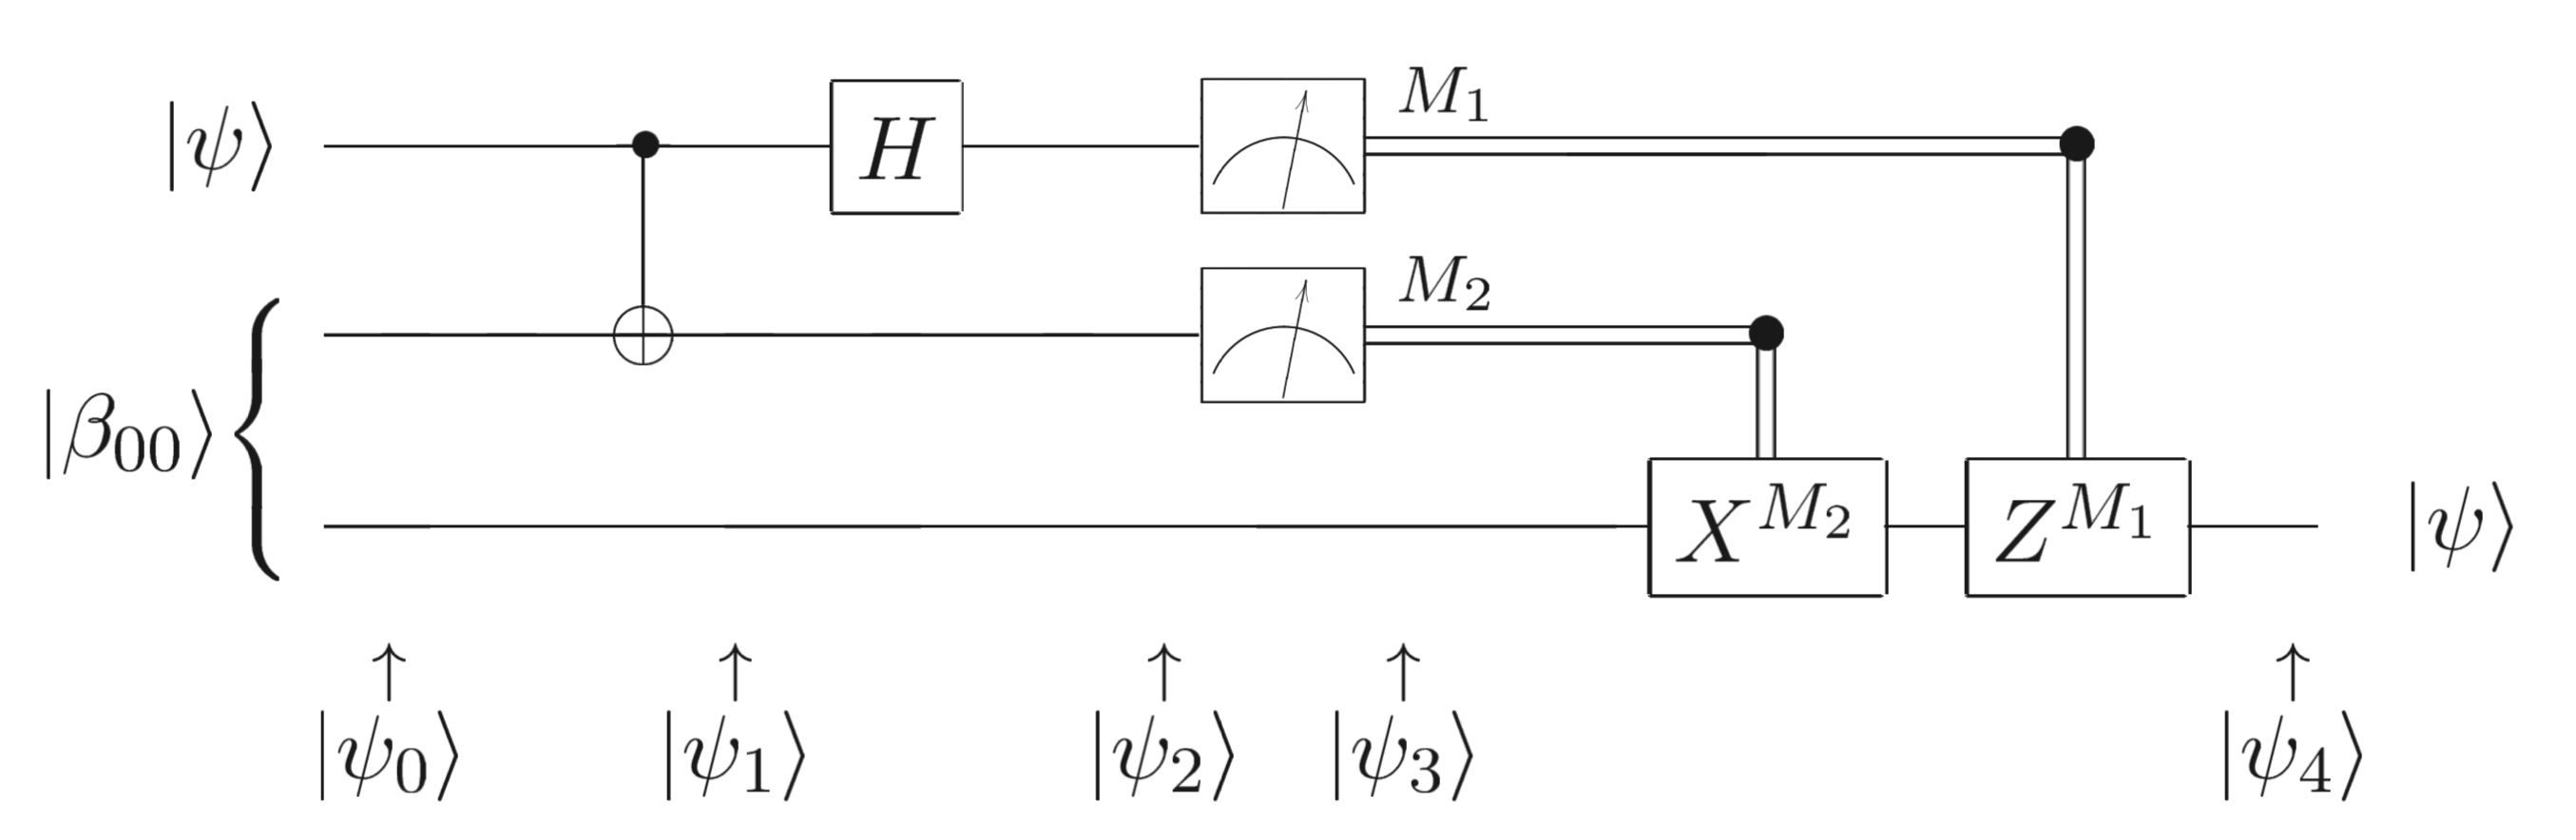
\includegraphics[width=\linewidth]{teleportation_circuit.png}	
\caption{Two top lines are Alice's system and bottom is Bob's}
\end{figure}

Recall the controlled-\texttt{NOT} (\texttt{CNOT}) takes $\ket{a}\ket{b}$ to $\ket{a}\ket{b \oplus a}$. The other gates in the circuit are summarized in the diagram below.

\begin{figure}[H]
\centering
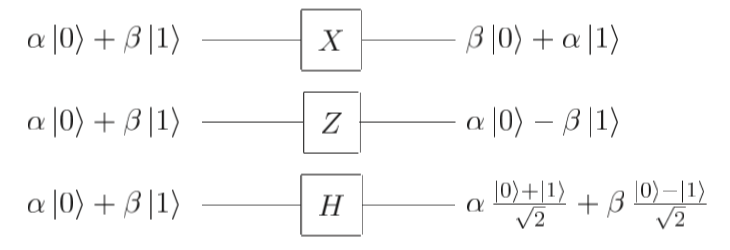
\includegraphics[width=0.5\linewidth]{basic_gates.png}	
\caption{Basic gates}
\end{figure}

So, the first two qubits belong to Alice and the third to Bob. Alice sends her qubits through a \texttt{CNOT} obtaining

\begin{align*}
\ket{\psi_1} &= \frac{1}{\sqrt{2}}\Big[\alpha\ket{0}(\ket{00} + \ket{11}) + \beta\ket{1}(\ket{10} + \ket{01})\Big]
\end{align*}

Then, Alice's first qubit is sent through a Hadamard gate which gives

\begin{align*}
\ket{\psi_2} &= \frac{1}{2}\Big[\alpha(\ket{0}+\ket{1})(\ket{00} + \ket{11}) + \beta(\ket{0}-\ket{1})(\ket{10} + \ket{01})\Big] \\
&= \frac{1}{2}\Big[ \ket{00} (\alpha\ket{0} + \beta\ket{1}) + \ket{01}(\alpha\ket{1} + \beta \ket{0}) + \ket{10}(\alpha\ket{0} - \beta\ket{1}) + \ket{11}(\alpha\ket{1} - \beta\ket{0}) \Big]
\end{align*}

Now, observe that each grouping in this expression has Alice's bits in a different state ($\ket{00},\ket{01},\ket{10},\ket{11}$), each of which Alice may observe after a measurement. Curiously, each of these groupings has a unique corresponding state for Bob's qubits. Hence, we know the state of Bob's qubits given knowledge of the outcome of Alice's measurement.

Furthermore, note that each of the possible states of Bob's qubits after Alice's measurements can be readily transformed to $\ket{\psi}$. Consider the four cases

\begin{enumerate}
\item Alice measures $00$. Hence, Bob's state is already $\ket{\psi}$. 
\item Alice measures $01$. Hence, Bob's state is $\alpha\ket{1} + \beta \ket{0}$. So, just apply the $X$ gate. 
\item Alice measures $10$. Hence, Bob's state is $\alpha\ket{0} - \beta\ket{1}$. So, just apply the $Z$ gate to flip the second sign. 
\item Alice measures $11$. Hence, Bob's state is $\alpha\ket{1} - \beta\ket{0}$. So, apply the $X$ gate to flip the bits, then the $Z$ gate to flip the second sign. 
\end{enumerate}

So that's what the notation in the circuit above means, we apply $X$ or $Z$ to Bob's qubits to recover $\ket{\psi}$ depending on the outcome of Alice's measurement.

Pretty cool, right? Let's look at this a level deeper using the density operator formalism we've developed. Each of the 4 cases have probability $\frac{1}{4}$ of occurring after the measurement. Hence, the density operator is given by

\begin{align*}
	\rho =& \frac{1}{4}\Big[ \ket{00}\bra{00} (\alpha\ket{0} + \beta\ket{1})(\alpha^*\bra{0} + \beta^*\bra{1}) + \ket{01}\bra{01}(\alpha\ket{1} + \beta \ket{0})(\alpha^*\bra{1} + \beta^* \bra{0}) \\
	&+ \ket{10}\bra{10}(\alpha\ket{0} - \beta\ket{1})(\alpha^*\bra{0} - \beta^*\bra{1}) + \ket{11}\bra{11}(\alpha\ket{1} - \beta\ket{0})(\alpha^*\bra{1} - \beta^*\bra{0}) \Big]
\end{align*}

So, the reduced density operator of Bob's system is

\begin{align*}
	\rho^B =& \frac{1}{4}\Big[ \bra{00}\ket{00} (\alpha\ket{0} + \beta\ket{1})(\alpha^*\bra{0} + \beta^*\bra{1}) + \bra{01}\ket{01}(\alpha\ket{1} + \beta \ket{0})(\alpha^*\bra{1} + \beta^* \bra{0}) \\
	&+ \bra{10}\ket{10}(\alpha\ket{0} - \beta\ket{1})(\alpha^*\bra{0} - \beta^*\bra{1}) + \bra{11}\ket{11}(\alpha\ket{1} - \beta\ket{0})(\alpha^*\bra{1} - \beta^*\bra{0}) \Big] \\
	=& \frac{1}{4}\Big[(\alpha\ket{0} + \beta\ket{1})(\alpha^*\bra{0} + \beta^*\bra{1}) + (\alpha\ket{1} + \beta \ket{0})(\alpha^*\bra{1} + \beta^* \bra{0}) \\
	&+ (\alpha\ket{0} - \beta\ket{1})(\alpha^*\bra{0} - \beta^*\bra{1}) + (\alpha\ket{1} - \beta\ket{0})(\alpha^*\bra{1} - \beta^*\bra{0}) \Big] \\
	=& \frac{1}{4}\Big[2(\alpha^*\alpha + \beta^*\beta)\ket{0}\bra{0} + 2(\alpha^*\alpha + \beta^*\beta)\ket{1}\bra{1}] \\
	=& \frac{I}{2}
\end{align*}
by $|\alpha|^2 + |\beta|^2 = 1$ and completeness.

Hence, the state of Bob's system after Alice has performed the measurement (but before Bob has learned the measurement result) is $I/2$ which has no dependence upon the state $\ket{\psi}$ being teleported. Therefore, any measurements performed by Bob will contain no information about $\ket{\psi}$, so information being communicated is dependent on the classical communication channel, implying that the speed of light limit is obeyed.

\subsection{The Schmidt Decomposition and purifications}

Schmidt Decomposition theorem says given a pure state $\ket{\psi}$ in a composite system $AB$, then there are orthonormal states $\ket{i_A}$ and $\ket{i_B}$ in $A$ and $B$, respectively, such that

\begin{align*}
\ket{\psi} = \sum_i \lambda_i \ket{i_A}\ket{i_B}	
\end{align*}

where $\lambda_i$ is nonnegative real and $\sum_i \lambda_i^2 = 1$.

One readily seen implication is that the spectra of $\rho^A$ and $\rho^B$ are the same, given a pure state in composite system $AB$. 

\begin{exercise}(2.76)
% TODO 2.76	
\end{exercise}

\begin{exercise}(2.77)
% TODO 2.77	
\end{exercise}

\begin{exercise}(2.78)
% TODO 2.78
\end{exercise}

A second technique is purification. Suppose we are given a state $\rho^A$ of system $A$. We can then introduce another system $R$ and define a pure state $\ket{AR}$ for the joint system $AR$ such that $\rho^A = \tr_R (\ket{AR}\bra{AR})$. $R$ is simply a reference and has no physical significance, the point is that we can associate pure states with mixed states.

\begin{exercise}(2.79)
% TODO 2.79	
\end{exercise}

\begin{exercise}(2.80)
% TODO 2.80	
\end{exercise}

\begin{exercise}(2.81)
% TODO 2.81
\end{exercise}

\begin{exercise}(2.82)
% TODO 2.82
\end{exercise}

\subsection{EPR and the Bell Inequality}  

Imagine we perform the following measurement. Charlie prepares a quantum system of two qubits in the state

\begin{align*}
\ket{\psi} = \frac{\ket{01} - \ket{10}}{\sqrt{2}}	
\end{align*}

He passes the first bit to Alice and second to Bob. They perform measurements of the following observables

\begin{align*}
Q &= Z_1 \\
R &= X_1 \\
S &= \frac{-Z_2-X_2}{\sqrt{2}} \\
T &= \frac{Z_2 - X_2}{\sqrt{2}}	
\end{align*}

Alice decides randomly to measure either $Q$ or $R$ once she receives the qubit and similarly Bob decides randomly whether to measure $S$ or $T$. They perform these measurements at the same time.

Hence, there are 4 combinations of Alice-Bob measurements. We can calculate and show that 

\begin{align*}
\langle QS \rangle &= \frac{1}{\sqrt{2}}\\	
\langle RS \rangle &= \frac{1}{\sqrt{2}}\\	
\langle RT \rangle &= \frac{1}{\sqrt{2}}\\	
\langle QT \rangle &= \frac{1}{\sqrt{2}}\\	
\end{align*}

\begin{proof}
% TODO fill in bell's calculations	
\end{proof}

And so $\langle QS \rangle + \langle RS \rangle + \langle RT \rangle - \langle QT \rangle = 2\sqrt{2}$. This violates Bell's inequality, derived in the text, which says that this value should never exceed 2. 

Bell's inequality requires assuming that $Q,R,S,T$ have definite values before the Alice-Bob measurements (realism). Additionally, we assumed that Alice performing the measurement does not influence the result of Bob's measurement (locality). Hence, at least one of these assumptions must be incorrect, since experimentation confirms this quantum picture.


\subsection{No-cloning Theorem}

It is impossible to copy an unknown quantum state.

\begin{proof}
Suppose we have a quantum machine with two slots labelled $A$ and $B$. Slot $A$ starts out with unknown state $\ket{\psi}$ which is two be copied to $B$. Assume that $B$ starts out with some pure state $\ket{s}$.

Hence, the initial state of the machine is $\ket{\psi}\ket{s}$. So, some unitary evolution $U$ now effects the copying procedure

\begin{align*}
	U(\ket{\psi}\ket{s}) = \ket{\psi}\ket{\psi}
\end{align*}
	
	Suppose this works for two particular states $\ket{\psi}$ and $\ket{\phi}$. Hence,
	
	\begin{align*}
		U(\ket{\psi}\ket{s}) = \ket{\psi}\ket{\psi} \\
		U(\ket{\phi}\ket{s}) = \ket{\phi}\ket{\phi}
	\end{align*}
	
	Hence, take the inner product of the two equations and 
	
	\begin{align*}
		(\bra{\phi}\ket{\psi}\bra{s}\ket{s})U^\dag U &= \bra{\phi}\ket{\psi} \\
		\bra{\psi}\ket{\phi}\bra{\psi}\ket{\phi} &= |\bra{\phi}\ket{\psi}|^2
	\end{align*}
	
	Hence, either $\bra{\phi}\ket{\psi}$ is 0 or 1. Thus, either $\ket{\psi} = \ket{\phi}$ (a contradiction to assuming they're distinct) or the two states are orthogonal.
	
	Therefore, a cloning device can only clone states which are orthogonal to one another and so a general quantum cloning device is impossible.  
\end{proof}

\section{Nielsen \& Chuang: Chapter 4}

\subsection{Single Qubit Operations}

A single qubit in the state $a \ket{0} + b \ket{1}$ can be visualized as a point $(\theta, \phi)$ on the unit sphere, where $a = \cos(\theta / 2), b = e^{i\phi}sin(\theta / 2)$. This is called the Bloch sphere representation and $(\cos \phi \sin \theta , \sin \phi \sin \theta, \cos \theta)$ is called the Bloch vector. 

\begin{exercise} (4.1) Find the points on the Bloch sphere which correspond to the normalized eigenvectors of the different Paul matrices. 
\begin{proof}
	
Recall that, from Exercise 2.11, $X$ has eigenvalues $\pm 1$ with respective eigevectors $\Big\{ \frac{1}{\sqrt{2}}\begin{bmatrix} 1 \\ 1 \end{bmatrix}, \frac{1}{\sqrt{2}}\begin{bmatrix} 1 \\ -1 \end{bmatrix} \Big\}$. Similarly, $Y$ has eigenvalues $\pm 1$ with respective eigenvectors $\Big\{ \frac{1}{\sqrt{2}}\begin{bmatrix} 1 \\ i \end{bmatrix} , \frac{1}{\sqrt{2}} \begin{bmatrix} 1 \\ -i \end{bmatrix} \Big\}$. Finally, $Z$ has eigenvalues $\pm 1$ with respective eigenvectors $\Big\{ \begin{bmatrix} 1 \\ 0 \end{bmatrix} , \begin{bmatrix} 0 \\ 1 \end{bmatrix} \Big\}$.
	
First, we solve for $X$. 
	
$\Big\{ \frac{1}{\sqrt{2}}\begin{bmatrix} 1 \\ 1 \end{bmatrix}, \frac{1}{\sqrt{2}}\begin{bmatrix} 1 \\ -1 \end{bmatrix} \Big\} \iff \{ \frac{1}{\sqrt{2}}(\ket{0} + \ket{1}) , \frac{1}{\sqrt{2}}(\ket{0} - \ket{1}) \} $. First, for $\frac{1}{\sqrt{2}}(\ket{0} + \ket{1})$, we have that $\cos(\theta / 2) = \frac{1}{\sqrt{2}}$. Hence, $\theta = \pi / 2$. Now, $e^{i\phi} \sin (\theta / 2) = e^{i \phi} / \sqrt{2} = 1 / \sqrt{2}$. Hence, $\phi = 0$. 
	
Similarly, for the second eigenvector, $\theta = \pi / 2$ but $\phi = - \pi$.
	
Therefore, for the first eigenvector, 
	
	\begin{align*}
	(\cos \phi \sin \theta , \sin \phi \sin \theta, \cos \theta) &= (\cos (0)\sin (\pi / 2) , \sin (0)\sin (\pi / 2) , \cos (\pi / 2) ) \\
	&= (1, 0, 0) \\
	\intertext{And for the second we have,}	
	(\cos (\pi)\sin (\pi / 2) , \sin (\pi)\sin (\pi / 2) , \cos (\pi / 2) ) \\
	&= (-1, 0, 0)
	\end{align*}

Similarly, we find the Bloch vectors $(0, \pm 1, 0)$ for $Y$ and $(0, 0, \pm 1)$ for $Z$.
\end{proof}
\end{exercise}

\subsubsection{Action by Hadamard on the Bloch Sphere}\label{had:bloch}

Note that the above exercise also shows that, on the Bloch sphere, $\ket{0} = (0, 0, 1), \ket{1} = (0, 0 , -1), \ket{+} = (1, 0, 0), \ket{-} = (-1, 0, 0)$. This can often aid intuition. For example, we know that Hadamard operator $H$ is defined s.t. $\ket{0} \rightarrow^{H} \ket{+}$. 

Hence, on the Bloch sphere, this transformation is equivalent to $(0, 0, 1) \rightarrow^{H} (1, 0, 0)$. So, we can define a series of rotations to emulate the action of $H$, by considering its action on a basis of the Bloch sphere. So we note the additional transformations, $H^2 = I \implies \ket{+} \rightarrow \ket{0} \iff (1, 0, 0) \rightarrow (0, 0, 1)$ and $H \begin{bmatrix} 1 \\ i \end{bmatrix} = \begin{bmatrix} 1 + i \\ 1 - i \end{bmatrix} = \begin{bmatrix} 1 \\ -i \end{bmatrix}$ (up to a global phase) $\iff$ $(0, 1, 0) \rightarrow (0, -1, 0)$.

Geometrically, we can convince ourselves that the following procedure suffices. For example, consider the effect of this procedure on $\ket{0}$:

(1) Begin with state $\ket{0} = (0,0,1)$

(2) Rotate by $- \pi / 2$ about the $\hat{x}$ axis. Hence, we then have $(0, 1,0)$.

(3) Rotate by $- \pi / 2$ about the $\hat{z}$ axis. This gives $(1, 0, 0)$.

(4) Rotate by $- \pi / 2$ about the $\hat{x}$ axis. This keeps us at $(1, 0, 0) = \ket{+}$

Similarly, using the same procedure

(1) $\begin{bmatrix} 1 \\ i \end{bmatrix} = (0, 1, 0)$.

(2) $(0, 0 , -1)$.

(3) $(0, 0, -1)$.

(4) $(0, -1, 0)$.

The reader can verify the above for $\ket{+}$. 

\begin{exercise} (4.2) Let $x \in \RR$ and $A$ be a matrix that satisfies $A^2 = I$. Show that 

\begin{align*}
\exp(i A x) = \cos(x) I + i \sin(x) A	
\end{align*}
 
\begin{proof}

From the power series definition of $e^{z}$, we have that
	
	\begin{align*}
		\exp(i A x) &=  \sum_{n=0}^\infty \frac{(iAx)^n}{n!} \\
		&= \sum_{n=0}^\infty \frac{(iAx)^{2n}}{(2n)!} + \sum_{n=0}^\infty \frac{(iAx)^{2n+1}}{(2n+1)!} \\
		\sum_{n=0}^\infty \frac{(iAx)^{2n}}{(2n)!} &= \sum_{n=0}^\infty \frac{i^{2n}A^{2n}x^{2n}}{(2n)!} \\
		&= \sum_{n=0}^\infty \frac{(-1)^{2n} I x^{2n}}{(2n)!} \\
		&= I \sum_{n=0}^\infty \frac{(-1)^{2n}  x^{2n}}{(2n)!} = \cos(x)I \\
		\sum_{n=0}^\infty \frac{(iAx)^{2n+1}}{(2n+1)!} &= \sum_{n=0}^\infty \frac{i^{2n+1}A^{2n+1}x^{2n+1}}{(2n+1)!} \\
		&= \sum_{n=0}^\infty \frac{i(-1)^{2n+1}Ax^{2n+1}}{(2n+1)!} \\
		&= iA \sum_{n=0}^\infty \frac{(-1)^{2n+1}x^{2n+1}}{(2n+1)!} = i\sin(x) A
	\end{align*}

\end{proof}
\end{exercise}

$X, Y, Z$ give rise to three useful classes of unitary matrices when they are exponentiated, the rotation operators about $\hat{x}$, $\hat{y}$, and $\hat{z}$,

\begin{align*}
R_x(\theta) \equiv e^{-i \theta X / 2} \\
R_y(\theta) \equiv e^{-i \theta Y / 2} \\
R_z(\theta) \equiv e^{-i \theta Z / 2} 
\end{align*}

We can use exercise 4.2 to write the above equations more conveniently.

\begin{exercise} (4.3) Show that, up to a global phase, the $\pi /8$ gate satisfies $T = R_z(\pi /4)$.

\begin{proof}

Note that 

$$
T = \begin{bmatrix}1 & 0 \\ 0 & \exp(i\pi / 4) \end{bmatrix} = \exp(i\pi / 8)\begin{bmatrix} \exp(-i \pi / 8)  & 0 \\ 0 & \exp(i \pi / 8)  \end{bmatrix} 
$$

Now, using the definition of $R_z$,

\begin{align*}
	e^{-i Z \frac{\pi}{8}} &= \cos(-\pi/8) I + i\sin (-\pi / 8)Z \\
	&=  \cos(\pi/8) I - i\sin (\pi / 8)Z \\
	&= \begin{bmatrix} \cos(\pi / 8) - i \sin (\pi / 8) & 0 \\ 0 & \cos(\pi/8) + i \sin (\pi / 8) \end{bmatrix} \\
	&= \begin{bmatrix} \exp(-i \pi / 8)  & 0 \\ 0 & \exp(i \pi / 8)  \end{bmatrix} \\
\end{align*}
\end{proof}
\end{exercise}

\begin{exercise} (4.4) Express the Hadamard gate $H$ as a product of $R_x$ and $R_z$ rotations and $e^{i \phi}$ for some $\phi $.
\begin{proof}

	In section \ref{had:bloch} we discussed a procedure for expressing $H$ as a product of rotations on the Bloch sphere, by considering its actions on a basis of the Bloch sphere. We showed that $R_x(-\pi / 2)R_z(-\pi / 2)R_x(-\pi / 2)$ suffices. We can verify this result a second way by considering the respective rotation matrices. 
	 
	We know that $H = \frac{1}{\sqrt{2}} (X + Z)$. Furthermore, 
	
	\begin{align*}
	R_x(-\pi / 2) &= \begin{bmatrix}
 \cos(\pi / 4) & i\sin(\pi / 4) \\ i\sin(\pi / 4) & \cos(\pi / 4)	
 \end{bmatrix} \\
&= \frac{1}{\sqrt{2}} \begin{bmatrix}
 	1 & i \\ i & 1 
 \end{bmatrix} = \frac{1}{\sqrt{2}}( I + iX) \\
 R_z(-\pi / 2) &= \begin{bmatrix}
 \cos(\pi / 4) + i\sin(\pi / 4) & 0 \\ 0 & \cos(\pi / 4)	 - i\sin (\pi / 4)
 \end{bmatrix} \\
&= \frac{1}{\sqrt{2}} \begin{bmatrix}
 	1 + i & 0 \\ 0 & 1-i
 \end{bmatrix} = \frac{1}{\sqrt{2}}( I + iZ)
\end{align*}

We'll use that 

\begin{align*}
XZ &= \begin{bmatrix}0 & 1 \\ 1 & 0\end{bmatrix}	\begin{bmatrix}1 & 0 \\ 0 & -1\end{bmatrix}	\\
&= \begin{bmatrix} 0 & -1 \\ 1 & 0 \end{bmatrix} = iY \\
ZX &= \begin{bmatrix}1 & 0 \\ 0 & -1\end{bmatrix}\begin{bmatrix}0 & 1 \\ 1 & 0\end{bmatrix} \\
&= \begin{bmatrix} 0 & 1 \\ -1 & 0 \end{bmatrix} = -iY \\
\implies XZ + ZX = 0 \\
\implies XZX + ZX^2 = 0 \\
\implies XZX = -Z 
\end{align*}

Note that the above is simply showing that the anti-commutator of $X$ and $Z$, $\{ X , Z\} = 0$. This holds for any pair of distinct Pauli matrices (Exercise 2.41). 

Hence,

\begin{align*}
	\frac{1}{2\sqrt{2}}( I + iX)( I + iZ)( I + iX) &= \frac{1}{2\sqrt{2}}[I + iX + iZ + i^2ZX + iX + i^2X^2 + i^2XZ + i^3XZX ]\\
	&= \frac{1}{2\sqrt{2}}[I + iX + iZ - ZX  + iX - I - XZ + i^3 XZX] \\
	&= \frac{1}{2\sqrt{2}}[i (X + Z)  + iX -i XZX ]\\
	&= \frac{1}{2\sqrt{2}}[i(X + Z) + iX + iZ ]\\
	&= \frac{1}{\sqrt{2}}[i(X + Z)]
\end{align*}

which gives the Hadamard transform with phase $e^{i0}$. 

\end{proof}
	
\end{exercise}


\begin{exercise} (4.5) Prove that $(\hat{n} \cdot \hat{\sigma} ) ^2 = I$, and use this to verify the following equation

\begin{align*}
R_n(\theta) \equiv \exp(-i \theta n \cdot \sigma / 2) = \cos(\theta /2) I - i \sin(\theta / 2) (n_x X + n_y Y + n_z Z) 	
\end{align*}

\begin{proof}

Evidently, $\hat{n} \cdot \hat{\sigma} = (n_x X + n_y Y + n_z Z)$ so, recalling that distinct Pauli matrices anti-commute,

\begin{align*}
(n_x X + n_y Y + n_z Z)^2 &= n_x^2X^2 + n_xn_y XY + n_x n_z XZ + n_xn_y YX + n_y^2 Y^2 + n_yn_z YZ + n_x n_z ZX + n_y n_z ZY + n_z Z^2 \\
&= (n_x^2 + n_y^2 + n_z^2)I + n_xn_z(XZ + ZX) + n_yn_z (YZ + ZY) + n_x n_y (XY + YX) \\
&= (n_x^2 + n_y^2 + n_z^2)I = I
\end{align*}

because $\hat{n}$ is a unit vector. 
	
Therefore, using Exercise 4.2 (Nielsen \& Chuang), if we let $A = \hat{n} \cdot \hat{\sigma}$, then the result follows directly.  
\end{proof}
\end{exercise}

% TODO 4.6
%\begin{exercise} (4.6) One reason why the $R_{\hat n} (\theta )$ operators are referred to as rotation operators is the following fact, which you are to prove. Suppose a single qubit has a state represented by the Bloch vector $\vec{\lambda}$. Then the effect of the rotation $R_{\hat n} (\theta )$ on the state is to rotate it by an angle $\theta$ about the $\hat{n}$ axis of the Bloch sphere. This fact explains the rather mysterious looking factor of two in the definition of the rotation matrices.

%\begin{proof}
%	The axis $v$ with which we rotate around is the vector that is unperturbed by action of $R_{\hat n} (\theta )$ i.e. $R_{\hat n} (\theta ) v = v$. Hence, $v$ is the eigenvector of $R_{\hat n} (\theta )$ with associated eigenvalue $1$. So, first we write the matrix
%	
%	\begin{align*}
%	R_{\hat n} (\theta ) &= \begin{bmatrix}
 %\cos(\theta / 2) - i n_z \sin(\theta / 2) & - (i n_x + n_y ) \sin(\theta / 2) \\ - (i n_x - n_y ) \sin(\theta / 2) & \cos(\theta / 2) 	+ i n_z \sin(\theta / 2)
 %\end{bmatrix}
%	\end{align*}
%
%Now, we solve for the eigenvector with eigenvalue $1$ which we assume to exist if this is a proper rotation matrix
%
%\begin{align*}
%	R_{\hat n} (\theta ) - I &= \begin{bmatrix}
 %\cos(\theta / 2) - i n_z \sin(\theta / 2) - 1 & - (i n_x + n_y ) \sin(\theta / 2) \\ - (i n_x - n_y ) \sin(\theta / 2) & \cos(\theta / 2) 	+ i n_z \sin(\theta / 2) - 1
 %\end{bmatrix} \\
 %0 &= \cos(\theta / 2)v_1 - i n_z \sin(\theta / 2)v_1 - v_1  - (i n_x + n_y ) \sin(\theta / 2)v_2  \\
 %0 &= - (i n_x - n_y ) \sin(\theta / 2)v_1 + \cos(\theta / 2)v_2 	+ i n_z \sin(\theta / 2)v_2 - v_2	
 %\end{align*}	
%\end{proof}
%\end{exercise}

\begin{exercise} (4.7) Show that $XY X = −Y$ and use this to prove that $XR_y(\theta)X = R_y(-\theta)$.

\begin{proof}
	From above, we have that distinct Pauli matrices anti-commute. Furthermore, the Pauli matrices are hermitian and unitary $\implies$ $\sigma_i^2 = 0, i \in \{x, y, z \}$. Hence, 
	
	\begin{align*}
	XY + YX &= 0 \\
	XYX + YX^2 &= 0 \\
	XYX + Y &=0 \\
	XYX &= -Y
	\end{align*}

So, 

\begin{align*}
XR_y(\theta)X &= X\big[\cos(\theta/2)I - i\sin(\theta / 2) Y\big]X \\
&= 	\cos(\theta/2)X^2 -i\sin(\theta/2)XYX \\
&= \cos(\theta/2)I + i \sin(\theta /2) Y \\
&= \cos(-\theta/2)I - i \sin(-\theta /2) Y \\
&= R_y(-\theta)
\end{align*}

using that $\cos(-x) = \cos(x), \sin(-x) = -\sin(x)$.
\end{proof}
\end{exercise}

% TODO 4.8
% TODO 4.9
% TODO 4.10
% TODO 4.11

\begin{lemma}\label{4.12}
Suppose $U$ is a unitary operation on a single qubit. Then there exist real numbers $\alpha, \beta, \gamma, \delta$ such that

\begin{align*}
	U = \begin{bmatrix}
 	e^{i(\alpha - \beta / 2 - \delta / 2)} \cos ( \gamma / 2) & -e^{i (\alpha - \beta /2 + \delta / 2)} \sin(\gamma / 2) \\ 
 	e^{i(\alpha + \beta / 2 - \delta / 2)} \sin ( \gamma / 2) & e^{i (\alpha + \beta /2 + \delta / 2)} \cos(\gamma / 2)
 \end{bmatrix}
\end{align*}
\end{lemma}

\begin{theorem}
Suppose $U$ is a unitary operation on a single qubit. Then there exist real numbers $\alpha, \beta, \gamma, \delta$ such that

$$
U = e^{i\alpha}R_z(\beta)R_y(\gamma)R_z(\delta).
$$	
\end{theorem}

\begin{corollary}\label{4.2}
	Suppose $U$ is a unitary gate on a single qubit. Then there exist unitary operators $A, B, C$ on a single qubit such that $ABC = I$ and $U = e^{i\alpha}AXBXC$, where $\alpha$ is some overall phase factor.
\end{corollary}

\begin{exercise} (4.12) Give $A, B, C$, and $\alpha$ for the Hadamard gate.

\begin{proof}
	Using Lemma \ref{4.12} above we can solve, assuming $\gamma = \pi / 2$, 
	\begin{align*}
		H &= \begin{bmatrix}
 1 & 1 \\ 1 & -1	
 \end{bmatrix} = \begin{bmatrix}
 	e^{i(\alpha - \beta / 2 - \delta / 2)} & -e^{i (\alpha - \beta /2 + \delta / 2)} \\ 
 	e^{i(\alpha + \beta / 2 - \delta / 2)} & e^{i (\alpha + \beta /2 + \delta / 2)}
 \end{bmatrix} \\ 
 \alpha - \beta / 2 - \delta / 2 &= 0 \\
 \alpha - \beta /2 + \delta / 2 &= \pi \\
 \alpha + \beta / 2 - \delta / 2 &= 0 \\
 (\alpha + \beta /2 + \delta / 2) &= \pi \\
 \implies \alpha &= \pi / 2, \beta = 0, \delta = \pi
	\end{align*}

So, the proof of Corollary \ref{4.2} in Nielsen \& Chuang tells us to set 

\begin{align*}
A &= R_z (\beta)R_y(\gamma / 2) \\
&= R_z (0)R_y(\pi / 4) \\
&= \begin{bmatrix}
 	\cos(\pi / 8) & -\sin(\pi / 8) \\
 	\sin(\pi / 8) & \cos(\pi / 8)
 \end{bmatrix}\\
B &= R_y(-\gamma/2)R_z(- (\delta+\beta)/2)\\
&= R_y(- \pi/4)R_z(- \pi/2)\\
&=  \begin{bmatrix}
 	\cos(\pi / 8) & \sin(\pi / 8) \\
 	-\sin(\pi / 8) & \cos(\pi / 8)
 \end{bmatrix} \begin{bmatrix}
 	e^{i\pi / 4} & 0 \\
 	0 & e^{- i\pi / 4}
 \end{bmatrix}\\
C &= R_z((\delta - \beta)/2)\\
&= R_z(\pi /2) \\
&= \begin{bmatrix}
 	e^{i\pi / 4} & 0 \\
 	0 & e^{- i\pi / 4}
 \end{bmatrix}\\
\end{align*}

and $\alpha$ remains set $\alpha = \pi / 2$.
\end{proof}	
\end{exercise}
% TODO 4.13
% TODO 4.14
% TODO 4.15

\subsection{Controlled Operations} 

In terms of the computational basis, the action of the \texttt{CNOT} is given by $\ket{c}\ket{t} \rightarrow \ket{c} \ket{t \oplus c}$.

\begin{exercise}(4.16)

What is the $4\times 4$ unitary matrix for the circuit

\begin{figure}[H]
\centering
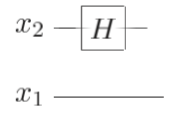
\includegraphics[width=.2\linewidth]{4_16-1.png}
\end{figure}

in the computational basis? What is the unitary matrix for the circuit

\begin{figure}[H]
\centering
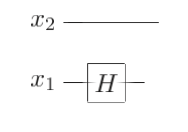
\includegraphics[width=.25\linewidth]{4_16-2.png}
\end{figure}

in the computational basis?

\begin{proof}
	For the first circuit, we consider action on the computational basis.
	
	\begin{align*}
		\ket{x_1}\ket{x_2 } &\rightarrow \ket{x_1}H\ket{x_2} = (I \otimes H) \ket{x_1}\ket{x_2 }
	\end{align*}

Now, given that $H = \begin{bmatrix} 1 & 1 \\ 1 & -1\end{bmatrix}$ w.r.t the computation basis, then

\begin{align*}
	(I \otimes H) &= \begin{bmatrix}	
	1 & 1 & 0 & 0 \\
	1 & -1 & 0 & 0 \\
	0 & 0 & 1 & 1 \\
	0 & 0 & 1 & -1
 \end{bmatrix}
\end{align*}

Similarly, for the second circuit we have

\begin{align*}
	(H \otimes I) &= \begin{bmatrix}	
	1 & 0 & 1 & 0 \\
	0 & 1 & 0 & 1 \\
	1 & 0 & -1 & 0 \\
	0 & 1 & 0 & -1
 \end{bmatrix}
\end{align*}
\end{proof}	
\end{exercise}

\begin{exercise} (4.17)
Construct a \texttt{CNOT} gate from one controlled-$Z$ gate, that is, the gate whose action in the computational basis is specified by the unitary matrix

$$
\begin{bmatrix}
1 & 0 & 0 & 0 \\
0 & 1 & 0 & 0 \\
0 & 0 & 1 & 0 \\
0 & 0 & 0 & -1		
\end{bmatrix}
$$

and two Hadamard gates, specifying the control and target qubits.

\begin{proof}
Recall that, in terms of the computational basis, the action of the \texttt{CNOT} is given by $\ket{c}\ket{t} \rightarrow \ket{c} \ket{t \oplus c}$ and that $Z = \begin{bmatrix} 1 & 0 \\ 0 & -1 \end{bmatrix}$.

We construct our algorithm by first making the observation that $H\ket{+} = \ket{0}$ and $H\ket{-} = \ket{1}$. Hence, beginning with state $\ket{c}\ket{t}$ we can initially apply $H$ to $\ket{t}$. Now, using the control-$Z$ gate with $\ket{c}$ as the control and $H\ket{t}$ as the target, we have two cases: 

(1) If $\ket{c = 1}$, then the second qubit will swap either from $\ket{+}$ to $\ket{-}$ or vis versa. Therefore, we can apply another Hadamard to the second qubit and have $\ket{t \oplus c}$ at the second qubit, as expected. The first qubit is unaltered, as expected.

(2) If $\ket{c = 1}$, then the second qubit will remain unchanged. Hence, if we apply another Hadamard to the second qubit, then $\ket{t}$ is recovered since $H^2 = I$. So, we have the expected behavior. 

In summary, we have the circuit, beginning with state $\ket{c}\ket{t}$:

(1) Apply $H$ to the second qubit

(2) Controlled-$Z$ with the first qubit as the control and second as the target 

(3) Apply $H$ to the second qubit. 
\end{proof}
\end{exercise}

From the next exercise, we'll see that it didn't actually matter whether we used the first or second qubit as control/target:

\begin{exercise}(4.18) Show that
	
\begin{figure}[H]
\centering
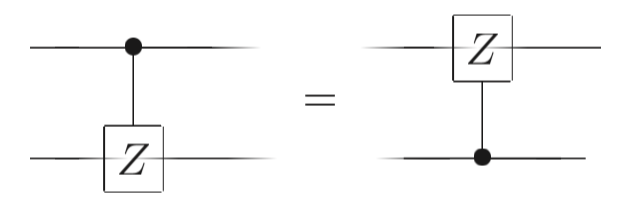
\includegraphics[width=.4\linewidth]{4_18.png}
\end{figure}

\begin{proof}
We simply prove the statement for the computational basis. 

(1) $\ket{0}\ket{0}$: Both circuits give the identity transform since they are conditioned on a qubit which is $\ket{0}$, in either case.

(2) $\ket{1}\ket{0}$: The first circuit is conditioned on $\ket{1}$, so it applies $Z$ to $\ket{0}$ which gives $\ket{0}$. Hence, we have $\ket{1}\ket{0}$. The second circuit is conditioned on $\ket{0}$, so we have the identity transform which gives $\ket{1}\ket{0}$, similarly.

(3) $\ket{0}\ket{1}$: By symmetry, we have the same outcome as in (2). 

(4) $\ket{1}\ket{1}$: The first circuit is conditioned on the first $\ket{1}$, so it applies $Z$ to the second qubit which gives $-\ket{1}\ket{1}$. Similarly, the second circuit gives $-\ket{1}\ket{1}$.
\end{proof}
\end{exercise}

\begin{exercise} (4.19) The \texttt{CNOT} gate is a simple permutation whose action on a density matrix $\rho$ is to rearrange the elements in the matrix. Write out this action explicitly in the computational basis.

\begin{proof}
	\begin{align*}
	\ket{00}\bra{00}  &= \begin{bmatrix}
 1 & 0 & 0 & 0 \\ 0 & 0 & 0 & 0 \\ 	0 & 0 & 0 & 0 \\ 0 & 0 & 0 & 0 
 \end{bmatrix} \\
 \ket{01}\bra{01}  &= \begin{bmatrix}
 0 & 0 & 0 & 0 \\  0 & 1 & 0 & 0 \\0 & 0 & 0 & 0 \\ 0 & 0 & 0 & 0 
 \end{bmatrix}\\
\ket{10}\bra{10}  &= \begin{bmatrix}
 0 & 0 & 0 & 0 \\  0 & 0 & 0 & 0 \\0 & 0 & 1 & 0 \\ 0 & 0 & 0 & 0  	
 \end{bmatrix} \\
 \ket{11}\bra{11}  &= \begin{bmatrix}
 0 & 0 & 0 & 0 \\  0 & 0 & 0 & 0 \\0 & 0 & 0 & 0 \\ 0 & 0 & 0 & 1
 \end{bmatrix}
	\end{align*}

Now, 

\begin{align*}
C_1(X)\ket{00} = \ket{00} \\
C_1(X)\ket{01} = \ket{01} \\
C_1(X)\ket{10} = \ket{11} \\
C_1(X)\ket{11} = \ket{10}
\end{align*}

Hence, the permutation matrix acting on the computational basis as

$$
\begin{bmatrix}
1 & 0 & 0 & 0 \\
0 & 1 & 0 & 0 \\
0 & 0 & 0 & 1 \\
0 & 0 & 1 & 0	
\end{bmatrix}
$$

satisfies this permutation. 
\end{proof}
\end{exercise}

\begin{exercise}(4.20) Unlike ideal classical gates, ideal quantum gates do not have (as electrical engineers say) ‘high-impedance’ inputs. In fact, the role of ‘control’ and ‘target’ are arbitrary – they depend on what basis you think of a device as operating in. We have described how the \texttt{CNOT} behaves with respect to the computational basis, and in this description the state of the control qubit is not changed. However, if we work in a different basis then the control qubit does change: we will show that its phase is flipped depending on the state of the ‘target’ qubit! Show that

\begin{figure}[H]
\centering
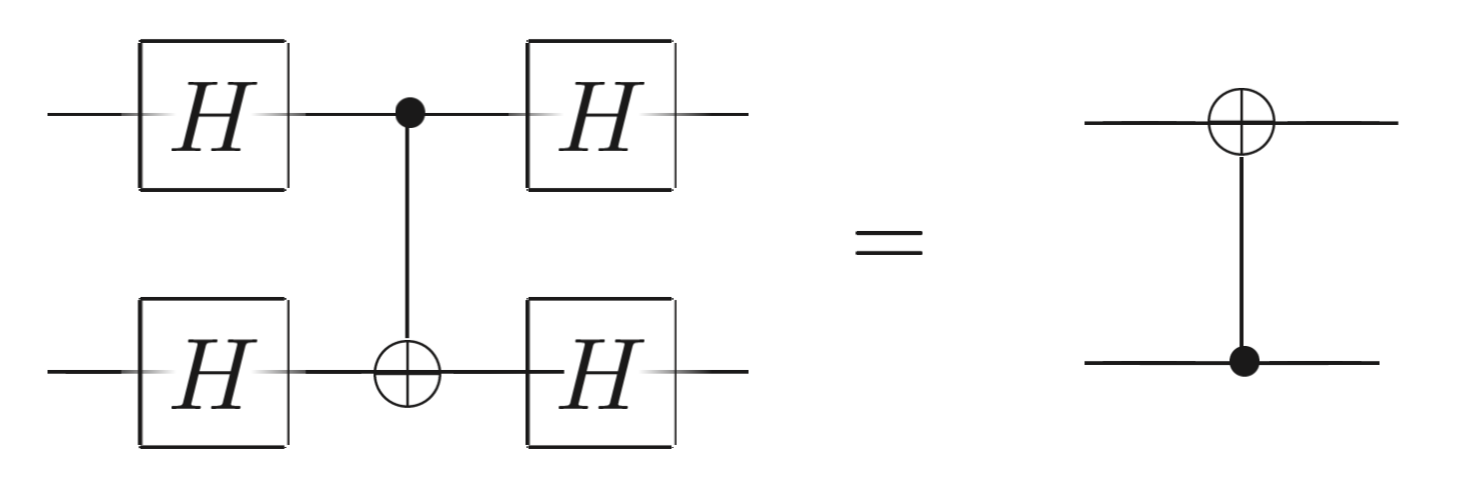
\includegraphics[width=.5\linewidth]{4_20.png}
\end{figure}

Introducing basis states $\ket{\pm}$ use this circuit identity to show that the effect of a \texttt{CNOT} with the first qubit as control and the second qubit as target is as follows:


\begin{align*}
\ket{+}\ket{+} \rightarrow \ket{+}\ket{+} \\	
\ket{-}\ket{+} \rightarrow \ket{-}\ket{+} \\	
\ket{+}\ket{-} \rightarrow \ket{-}\ket{-} \\	
\ket{-}\ket{-} \rightarrow \ket{+}\ket{-} 
\end{align*}

Thus, with respect to this new basis, the state of the target qubit is not changed, while the state of the control qubit is flipped if the target starts as $\ket{-}$, otherwise it is left alone. That is, in this basis, the target and control have essentially interchanged roles!

\begin{proof}
Consider action on $\ket{c}\ket{t}$ by the circuit on the LHS. The action of this circuit is given by $(H \otimes H) C^1(X)\ket{c}\ket{t} (H \otimes H)$ using $c$ as the control and $t$ as the target for the controlled operation. So, in Exercise 4.17, we showed that we can decompose $C^1(X)$ as $HC^1(Z)H$ using the same control and target as used for $C^1(X)$ originally, and with the $H$ transforms acting on the target qubit. Hence, we can rewrite action by the LHS circuit as $(H \otimes H) (I \otimes H) C^1(Z)\ket{c}\ket{t} (I \otimes H) (H \otimes H) = (H \otimes I) C^1(Z)\ket{c}\ket{t} (H \otimes I)$.

Similarly, for the circuit on the RHS, action on $\ket{c}\ket{t}$ is given by $C^1(X)\ket{c}\ket{t}$ where in this case $t$ is the control and $c$ is the target. Hence, using the same result, we can rewrite this as $(H \otimes I) C^1(Z)\ket{c}\ket{t} (H \otimes I)$ with $t$ as control and $c$ as target. Finally, using Exercise 4.18, we can swap which qubits we regard as control/target in a controlled-$Z$ operation. Hence, we have the action $(H \otimes I) C^1(Z)\ket{c}\ket{t} (H \otimes I)$ with $c$ as control and $t$ as target, as in the LHS. 

Now, using that $H^2 = I$, we note that the identity given by the circuit is equivalent to $C^1(X) (H \otimes H)\ket{c}\ket{t} = C^1(X) \ket{t}\ket{c} (H \otimes H)$ (applying $H \otimes H$ to the end of both circuits). Hence, this directly gives the effect of \texttt{CNOT} on the basis $\ket{\pm}$. 

\end{proof}

\end{exercise}

\begin{exercise}(4.21) Verify that Figure 4.8 implements the $C^2(U)$ operation.
	
	\begin{proof}
		
	\end{proof}

\end{exercise}

%\begin{exercise}(4.23) Prove that a $C^2(U)$ gate (for any single qubit unitary $U$) can be
%constructed using at most eight one-qubit gates, and six controlled-\texttt{NOT}s.
%	
%	\begin{proof}
%	From Corollary \ref{4.2} we can decompose $U$ as $U = e^{i\alpha}AXBXC$. So, consider the circuit below
%	
%	\begin{figure}[H]
%\centering
%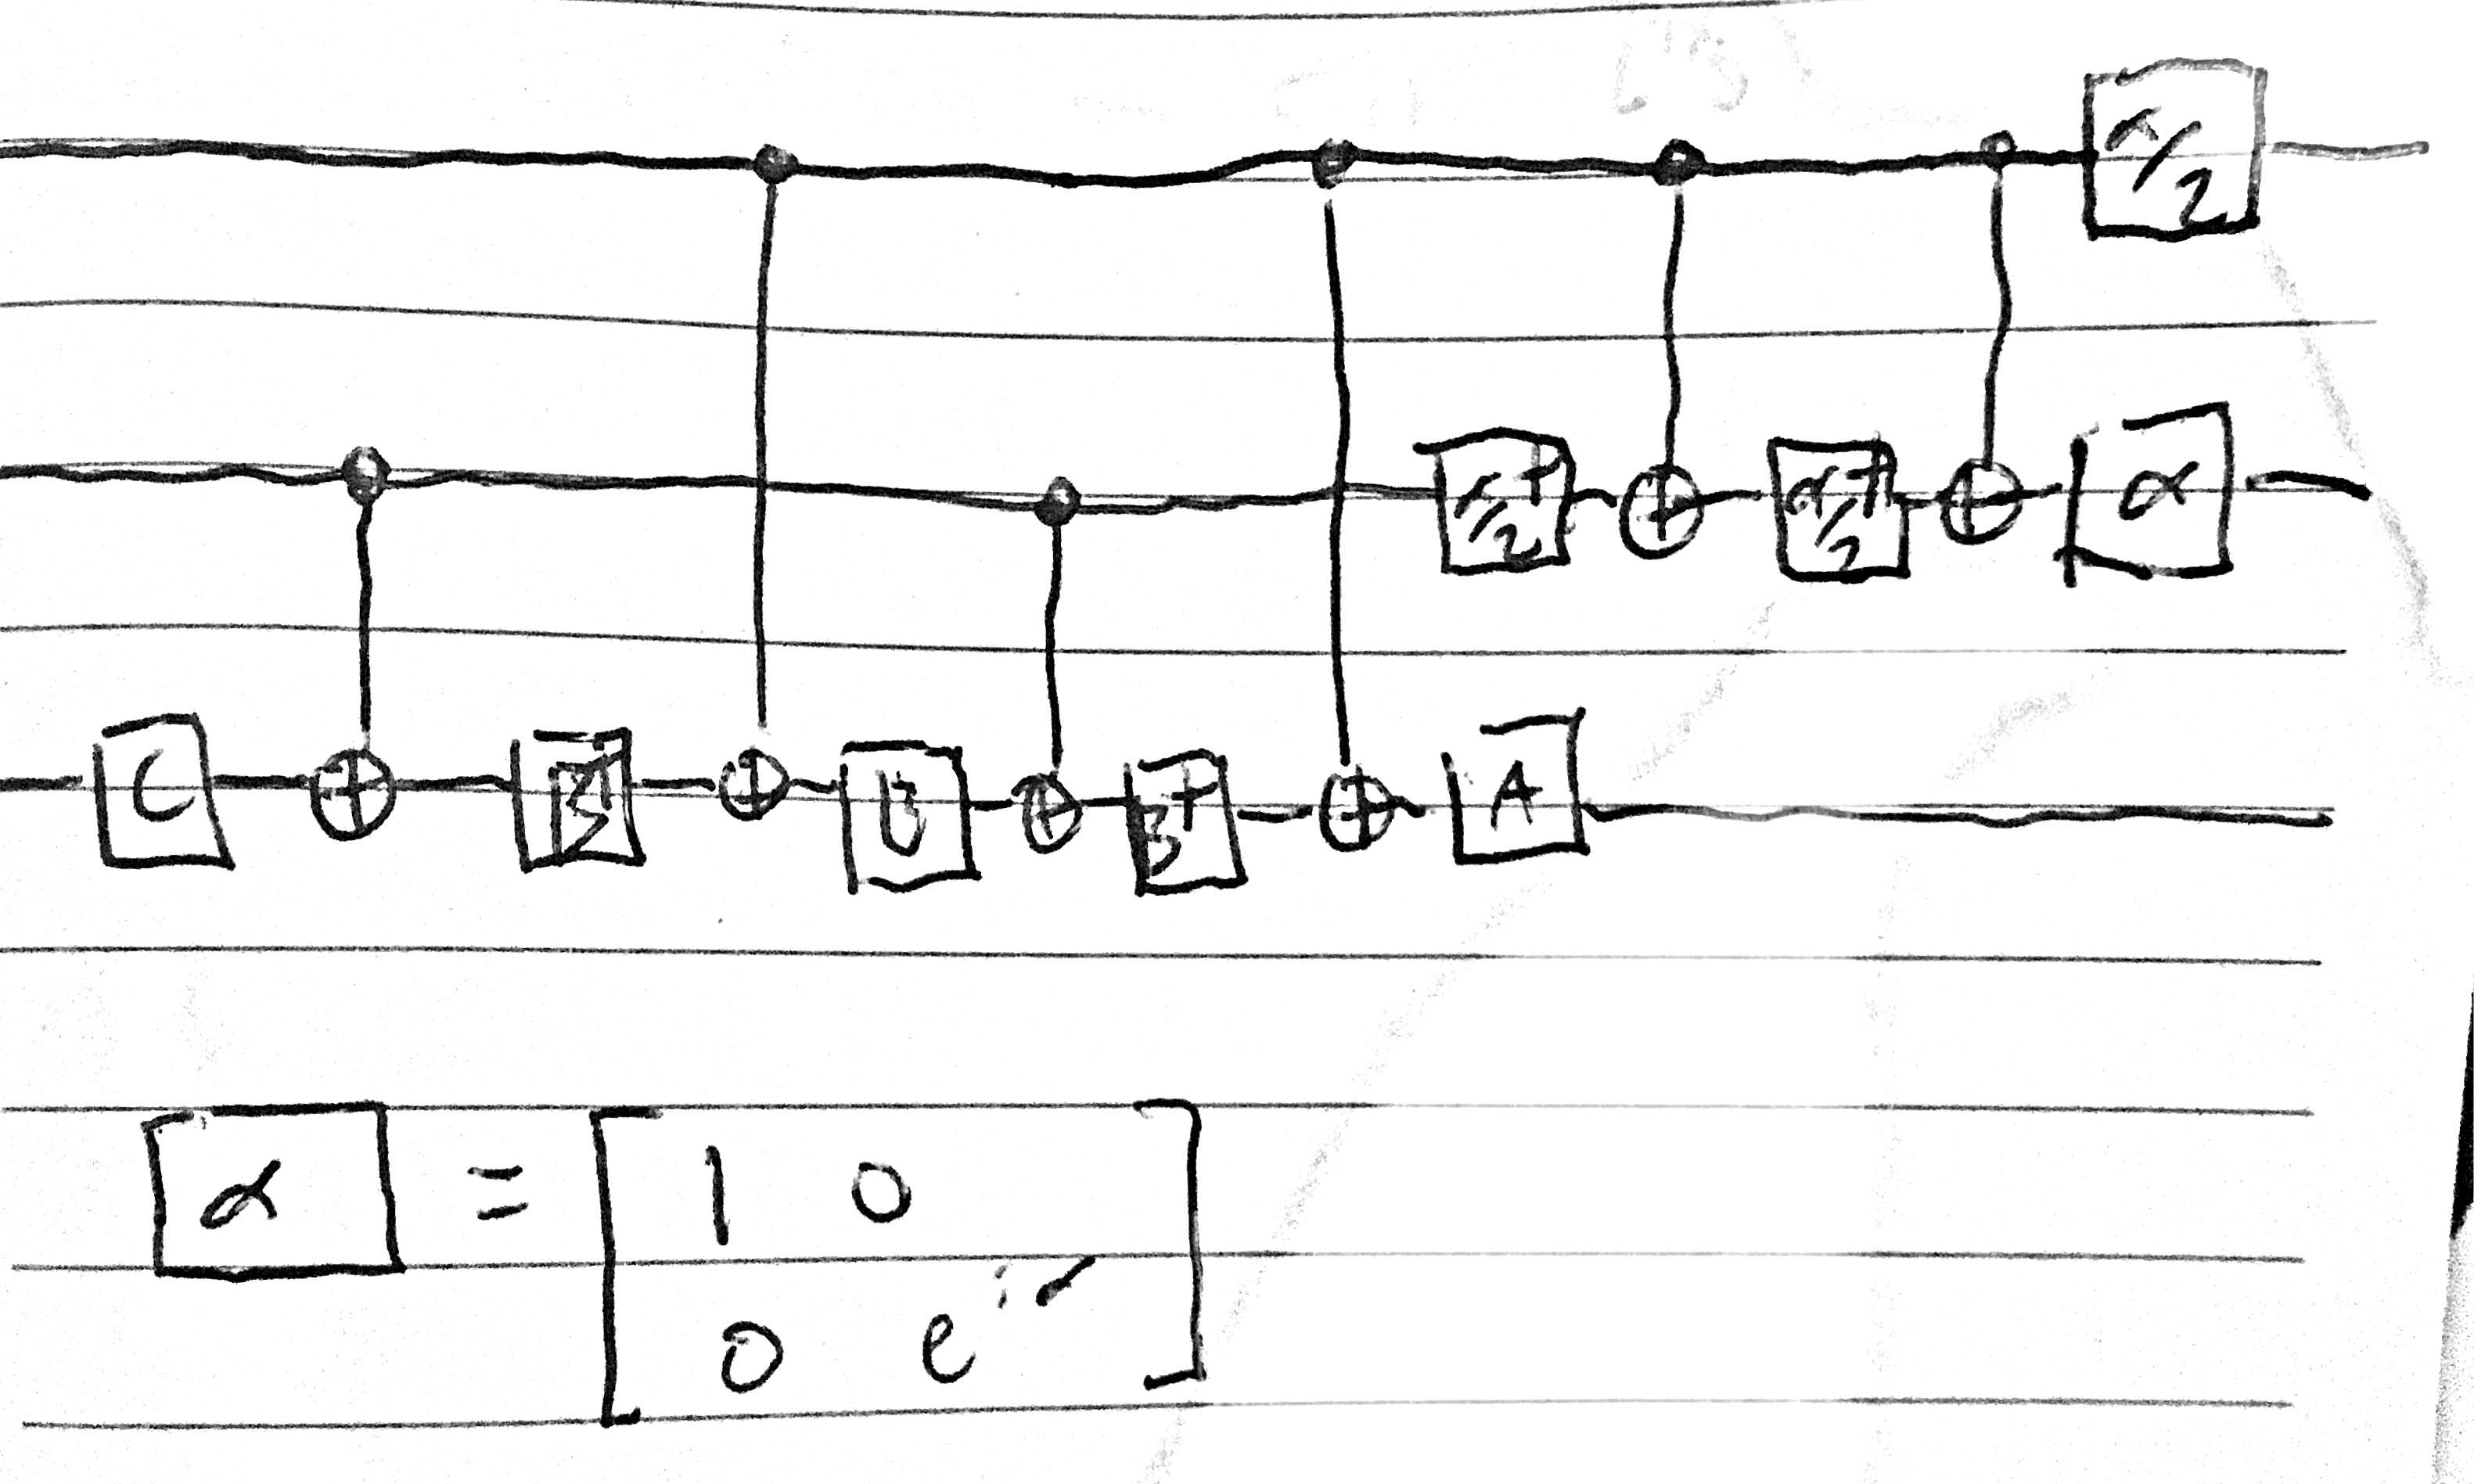
\includegraphics[width=0.75\linewidth]{4_23.jpg}	
%\end{figure}
%
%Label the qubits $x_0, x_1, x_2$ from bottom to top. So, first consider the effect of the circuit on the first qubit, $x_0$. 
%
%Hence, the circuit gives the transformation
%
%\begin{align*}
%	\ket{x_0} \mapsto AX^{x_2}B X^{x_1} B^\dag X^{x_2} B X^{x_1} C \ket{x_0}
%\end{align*}
%
%Therefore, we consider this action in the computation basis. Using that $ABC = I$ and $A,B, C$ are unitary we have
%
%\begin{align*}
%	x_1 = x_2 = 0 : \ket{x_0} &\mapsto AX^{0}B X^{0} B^\dag X^{0} B X^{0} C \ket{x_0} \\
%	&= ABB^\dag BC = ABC = I \\
%	x_1 = 1, x_2 = 0 : \ket{x_0} &\mapsto AX^{0}B X^{1} B^\dag X^{0} B X^{1} C \ket{x_0} \\
%	&= ABXB^\dag BXC = ABC = I \\
%	x_1 = 0, x_2 = 1 : \ket{x_0} &\mapsto AX^{1}B X^{0} B^\dag X^{1} B X^{0} C \ket{x_0} \\
%	&= AXBB^\dag XBC = ABC = I \\
%\end{align*}
%
%as expected.
%
%Now, for $x_1 = x_2 = 1$, we first recall that $B \equiv R_y(-\gamma / 2)R_z(-\frac{\delta + \beta}{2})$ from the proof of Corollary \ref{4.2}. Furthermore, from Exercise 4.7, $XBX = R_y(\gamma / 2)R_z(\frac{\delta + \beta}{2})$. Hence,
%
%\begin{align*}
%	B^\dag XBX &= R_z^\dag\Big(-\frac{\delta + \beta}{2}\Big)R_y^\dag(-\gamma / 2)R_y(\gamma / 2)R_z\Big(\frac{\delta + \beta}{2}\Big) \\
%	&= R_z\Big(-\frac{\delta + \beta}{2}\Big)R_y(-\gamma / 2)R_y(\gamma / 2)R_z\Big(\frac{\delta + \beta}{2}\Big) \\
%	R_z\Big(-\frac{\delta + \beta}{2}\Big)R_y(0)R_z\Big(\frac{\delta + \beta}{2}\Big) \\
%	&= R_z(0) = I
%\end{align*}
%
%Therefore,
%
%\begin{align*}
%	x_1 = 1, x_2 = 1 : \ket{x_0} &\mapsto AX^{1}B X^{1} B^\dag X^{1} B X^{1} C \ket{x_0} \\
%	&= AXBXB^\dag XBXC \\
%	&= AIXBXC = AXBXC
%\end{align*}
%
%which give $U$ up to a global phase. 
%
%Now, we consider the effect of the phase gates, $T_\alpha, T_{\alpha/2}$, on the global phase. 
%
%First, note that 
%
%\begin{align*}
%T_{\alpha/2}^\dag X T_{\alpha/2} X T_\alpha &= \begin{bmatrix}
% 	e^{-i\phi / 2} & 0 \\ 0 & e^{i \phi / 2} & 0
% \end{bmatrix} \\
% T_{\alpha/2}^\dag T_{\alpha/2} T_\alpha &= I 
%\end{align*}
%
%Hence, 
%
%\begin{align*}
%	\ket{x_1}\ket{x_2} \begin{bmatrix}
% 	e^{-i\phi / 2} & 0 \\ 0 & e^{i \phi / 2} & 0
% \end{bmatrix}\ket{x_1} \mapsto e^{i \frac{\phi}{2} x_2}\ket{x_2}
%\end{align*}
%
%Therefore, in the computational basis
%
%\begin{align*}
%x_1 = 0, x_2 = 0 : \ket{x_1}\ket{x_2} \mapsto 	
%\end{align*}
%\end{proof}
%\end{exercise}


\begin{exercise}
	
\end{exercise}

\subsection{Universal quantum gates}

A set of gates is said to be universal for quantum computation if any unitary operation may be approximated to arbitrary accuracy by a quantum circuit only involving those gates. We can show

(1) An arbitrary unitary operator may be expressed exactly as a product of unitary operators that each acts non-trivially only on a subspace spanned by two computational basis states

(2) An arbitrary unitary operator may be expressed exactly using single qubit and \texttt{CNOT} gates.

(3) Any unitary operation can be approximated to arbitrary accuracy using Hadamard, phase, \texttt{CNOT}, and $\pi / 8$ gates.

We are showing existence not efficiency.

\section{Nielsen \& Chuang: Chapter 5}

\subsection{Quantum Fourier Transform}

The quantum fourier transform on an orthonormal basis $\ket{0}, \cdots ,\ket{N - 1}$ is defined to be a linear operator with the following action on the basis states,

\begin{align*}
\ket{j} \rightarrow \frac{1}{\sqrt{N}} \sum_{k=0}^{N-1} e^{2\pi i jk / N} \ket{k}	
\end{align*}


\begin{exercise}(5.2) Explicitly compute the Fourier transform of the $n$ qubit state $\ket{00\cdots 0}$.
\begin{proof}
	$\ket{00 \cdots 0 }$ corresponds to state $\ket{0}$ in the size $N = 2^n$ computational basis. Hence, using the formula above we have 
	
	\begin{align*}
	\ket{0} &\rightarrow \frac{1}{\sqrt{N}} \sum_{k=0}^{N-1} \ket{k} \\
	&= 	\frac{\ket{0} + \ket{1} + \cdots + \ket{N-1}}{\sqrt{N}}
	\end{align*}

\end{proof}
	
\end{exercise}

We can derive an alternative product representation of the quantum fourier transform. First, represent some state $\ket{j}$ using its binary representation $j=j_1j_2 \cdots j_n$, $j_i \in \{0, 1\}$. Then,

\begin{align*}
\ket{j_1 , \cdots , j_n } \rightarrow \frac{(\ket{0} + e^{2\pi i 0.j_n} \ket{1})(\ket{0} + e^{2\pi i 0.j_{n-1}j_n} \ket{1})\cdots (\ket{0} + e^{2\pi i 0.j_1j_2 \cdots j_n} \ket{1})}{2^{n/2}}
\end{align*}

So, define the unitary transformation

\begin{align}
	R_k = \begin{bmatrix}
 1 & 0 \\ 0 & e^{2\pi i / 2^k}	
 \end{bmatrix}
\end{align}

Then, using the circuit below, we can see that this transformation is correctly implemented.

\begin{figure}[H]
\centering
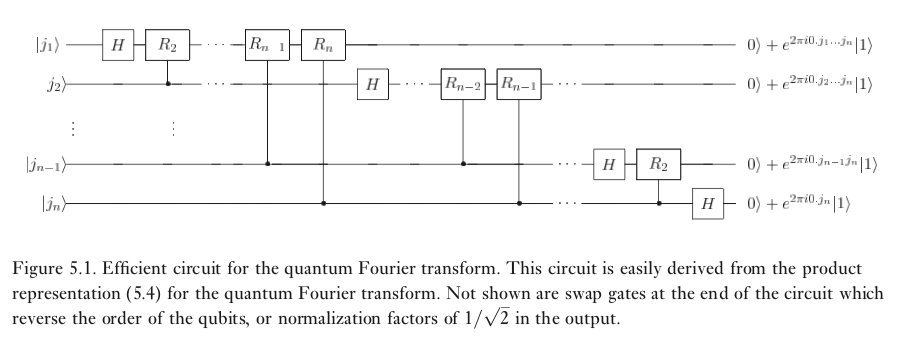
\includegraphics[width=\linewidth]{qfft.png}	
\end{figure}

Furthermore, the gate complexity is $O(n^2)$ as opposed to $O(n2^n)$, classically. 

\subsection{Quantum Phase Estimation Algorithm}\label{phase_estimation}

Suppose a unitary operator $U$ has an eigenvector $\ket{u}$ with eigenvalue $e^{2\pi i \phi}$, where the value of $\phi$ is unknown. 

\begin{figure}[H]
\centering
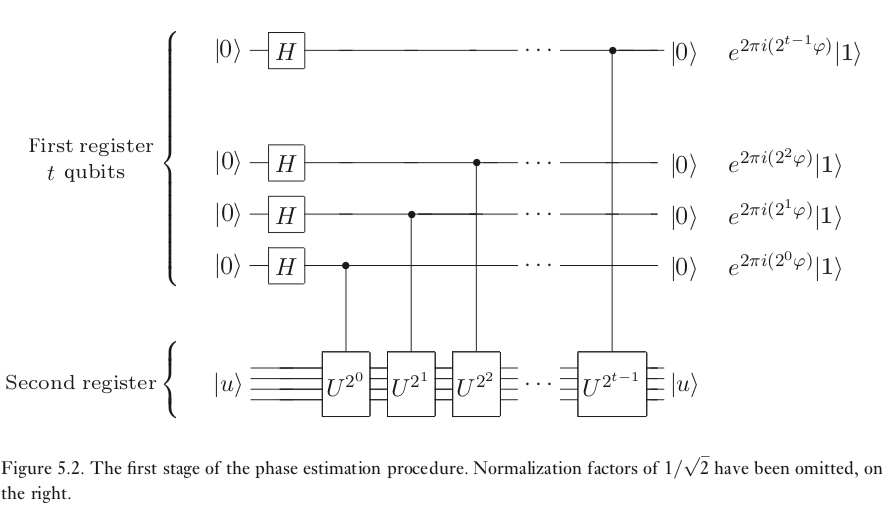
\includegraphics[width=\linewidth]{phase_estim.png}	
\end{figure}

Then, observe that the circuit above gives the state 

\begin{align*}
\frac{1}{2^t}(\ket{0} + e^{2 \pi i 0.\phi_t}\ket{1})(\ket{0} + e^{2 \pi i 0.\phi_{t-1}\phi_t}\ket{1})	\cdots (\ket{0} + e^{2 \pi i 0.\phi_1\phi_2\cdots\phi_t}\ket{1})	
\end{align*}

Hence, we can apply the inverse QFT and get the state $\ket{\phi_1 \cdots \phi_t}$, which is an approximation of $\phi$. 

\begin{exercise}(5.7) Additional insight into the circuit above may be obtained by showing, as you should now do, that the effect of the sequence of controlled-$U$ operations like that in the figure is to take the state $\ket{j}\ket{u}$ to $\ket{j} U^j\ket{u}$. (Note that this does not depend on $\ket{u}$ being an eigenstate of $U$.)
\begin{proof}
	Consider an arbitrary $j$ in its binary representation $j_0j_1 \cdots j_{t-1}$ where $j_i \in \{ 0, 1\}$. Hence, for each $\ket{j_i}$, the control-$U$ acts on $\ket{j_i}\ket{u}$ such that $\ket{j_i}\ket{u} \mapsto \ket{j_i}U^{j_i 2^i}\ket{u}$. Therefore, the final state is given by
	
	\begin{align*}
	\ket{j_0 } \cdots \ket{j_{t-1}}U^{j_0 2^0} \cdots U^{j_{t-1} 2^{t-1}}\ket{u} &= \ket{j} U^{j_0 2^0} \cdots U^{j_{t-1} 2^{t-1}}\ket{u} \\
	&= \ket{j} U^{j_0 2^0 + j_{t-1} 2^{t-1}}\ket{u} \\
	&= \ket{j} U^{j}\ket{u}
	\end{align*}
\end{proof}
\end{exercise}

\subsection{Order-Finding and Factoring}

\section{Nielsen \& Chuang: Chapter 6}

\subsection{The quantum search algorithm}

The Grover iteration may be broken up into four steps.

(1) Apply the oracle $O$

(2) Apply the Hadamard transform $H^{\otimes n}$

(3) Perform the conditional phase shift on the computer, with every computational basis
state except $\ket{0}$ receiving a phase shift of $-1$,

$$ \ket{x} \rightarrow -(-1)^{\delta x_0} \ket{x} $$

(4) Apply the Hadamard transform $H^{\otimes n}$

\begin{exercise}(6.1) Show that the Unitary operator corresponding to the phase shift in the Grover iteration is $2 \ket{0}\bra{0} - I$.
	\begin{proof}
	Consider arbitrary state $\ket{x}$. There are two cases:
	
	(1) $\ket{x} = \ket{0}$. Hence, 
	
	\begin{align*}
 	(2 \ket{0}\bra{0} - I)\ket{0} &= 2\ket{0}\bra{0}\ket{0} - \ket{0} \\
 	&= \ket{0}
 \end{align*}

as expected.

(2) $\ket{x} \neq \ket{0}$. Hence, 
	
	\begin{align*}
 	(2 \ket{0}\bra{0} - I)\ket{x} &= 2\ket{0}\bra{0}\ket{x \neq 0} - \ket{x} \\
 	&= 0 - \ket{x} = -\ket{x}
 \end{align*}

as expected.
	\end{proof}

\end{exercise}

\begin{exercise}(6.2) Show that the operation $(2 \ket{\psi}\bra{\psi} - I)$ (where $\ket{\psi}$ is the equally weighted superposition of states) applied to general state $\sum_k \alpha_k \ket{k}$ produces 

\begin{align*}
\sum_k [ -\alpha_k + 2\langle \alpha \rangle ] \ket{k}	
\end{align*}
	
	where $\langle \alpha \rangle \equiv \sum_k \alpha_k / N$ is the mean value of $\alpha_k$. 
	
	\begin{proof}
		\begin{align*}
			(2 \ket{\psi}\bra{\psi} - I) \sum_k \alpha_k \ket{k} &= \Big(2\frac{1}{N^{1/2}}\ket{x} \frac{1}{N^{1/2}} \sum_{x'=0}^{N-1} \bra{x'} - I\Big)\sum_k \alpha_k \ket{k} \\
			&= 2\frac{1}{N} \sum_{x=0}^{N-1} \ket{x}\bra{x'}\sum_k \alpha_k \ket{k} -\sum_k \alpha_k \ket{k} \\
			&= \frac{2}{N} \sum_k \ket{k}  \alpha_k -\sum_k \alpha_k \ket{k} \\
			&= \sum_k [ 2\langle \alpha \rangle -\alpha_k ] \ket{k}
		\end{align*}

	\end{proof}

\end{exercise}


\section{Algorithms for solving linear systems of equations}

One such application of Phase Estimation (Section \ref{phase_estimation}) is with respect to solving linear systems of equations. This is the so-called HHL algorithm \cite{lloyd2010quantum}.

The general problem statement of a linear system is if we are given matrix $A$ and unit vector $\vec{b}$, then find $\vec{x}$ satisfying, $A\vec{x} = \vec{b}$. 

However, assume that instead of solving for $x$ itself, we instead solve for an expectation value $x^T M x$ for some linear operator $M$. Hence, one can show that our algorithm has a runtime bound of $O(\log(N)\kappa ^{2})$, if we can further assume that the linear system is sparse and has a low condition number $\kappa$.

So, assume that $A$ in our linear system is an $N \times N$ Hermitian matrix. Notice that this is an "unrestrictive" constraint on $A$ because we can always take non-Hermitian matrix $A'$ and linear system $A' \vec{x} = \vec{b}$ and instead solve $\begin{bmatrix}
	0 && A' \\ A'^\dag && 0
\end{bmatrix} \begin{bmatrix} 0 \\ x \end{bmatrix} = \begin{bmatrix} b \\ 0 \end{bmatrix}$. Hence, we we will assume that $A$ is Hermitian from here on. 

Recall that because $A$ is hermitian $\implies$ we can perform quantum phase estimation using $e^{-iAt}$ as the unitary transformation. This can be done efficiently if $A$ is sparse.

So, we first prepare $\ket{b}$ (the representation of $\vec{b}$). We assume that this can be done efficiently or that $\ket{b}$ is supplied as an input.

Denote by $\ket{\psi_j}$ the eigenvectors of $A$ with associated eigenvalues $\lambda_j$. Hence, we can express $\ket{b}$ as $\ket{b} = \sum_j \beta_j \ket{\psi_j}$.  So, we initialize a first register to state $\sum_j \beta_j \ket{\psi_j}$ and second register to state $\ket{0}$ . After applying phase estimation, we then have the joint state $\sum_j \beta_j \ket{\psi_j} \ket{\widetilde{\lambda}_j}$, where $\widetilde{\lambda}_j$ is an approximation of $\lambda_j$. We'll assume that this approximation is perfect from here on. 

Next we add an ancilla qubit and perform a rotation conditional on the first register while now holds $\ket{\lambda_j}$. The rotation transforms the system to

\begin{align*}
\sum_j \beta_j \ket{\psi_j} \ket{\lambda_j} \Big(\sqrt{1-\frac{C^2}{\lambda_j^2}}\ket{0} + \frac{C}{\lambda_j}\ket{1}\Big)
\end{align*}

for some small constant $C \in \RR$ that is $O(1/\kappa)$.

Hence, we can undo phase estimation to restore the second register to $\ket{0}$.

Now, if we measure the ancillary qubit in the computational basis, we'll evidently collapse the state to $\ket{1}$ with some probability. We'd then have

\begin{align*}
	\sum_j \frac{C}{\lambda_j} \beta_j \ket{\psi_j} \ket{\lambda_j}\ket{1} = C (A^{-1} \ket{b})
\end{align*}

In particular, the probability of getting this result is 

\begin{align*} 
	p(-1) &= \Bigg(\sum_j \beta_j \bra{\psi_j} \bra{\lambda_j} \Big(\sqrt{1-\frac{C^2}{\lambda_j^2}}\bra{0} + \frac{C}{\lambda_j}\bra{1}\Big) \Bigg)\ket{1}\bra{1} \Bigg(\sum_j \beta_j \ket{\psi_j} \ket{\lambda_j} \Big(\sqrt{1-\frac{C^2}{\lambda_j^2}}\ket{0} + \frac{C}{\lambda_j}\ket{1}\Big)\Bigg) \\
	&= \sum_j \beta_j \bra{\psi_j} \bra{\lambda_j} \Big(\sqrt{1-\frac{C^2}{\lambda_j^2}}\bra{0} + \frac{C}{\lambda_j}\bra{1}\Big) \ket{1}\bra{1} \beta_j \ket{\psi_j} \ket{\lambda_j} \Big(\sqrt{1-\frac{C^2}{\lambda_j^2}}\ket{0} + \frac{C}{\lambda_j}\ket{1}\Big) \\
	&= \sum_j \beta_j \bra{\psi_j} \bra{\lambda_j} \frac{C}{\lambda_j}\bra{1}\ket{1}\bra{1} \beta_j \ket{\psi_j} \ket{\lambda_j} \frac{C}{\lambda_j}\ket{1} \\
	&= \sum_j \beta_j^2 \frac{C^2}{\lambda_j^2} \\
	&= \| A^{-1} \ket{b} \|^2 C^2 = O(1/\kappa^4)
\end{align*} 

Finally, we can make a measurement $M$ whose expectation value $\bra{x}M\ket{x}$ corresponds to the feature of $x$ we wish to evaluate. 

\section{Supervised learning with quantum enhanced feature spaces}

\subsection{Prelude}

We are given data from a training set $T$ and a test set $S$ of a subset $\Omega \subset \RR^d$. We assume that $S$ and $T$ are drawn from the same input space $X$. Furthermore, there exists output space $Y = \{ -1, +1 \} $ and a distribution $D$ on $X \times Y$.

Now, suppose we have a labelling $m: T \cup S \rightarrow Y$.  Our goal is to use this information to find some approximation function $\tilde{f} : X \rightarrow Y$ that minimizes estimation error for function class $F$. In other words, let true risk for function $f$ be defined as

\begin{align*}
R^{true}(f) = P_{X, Y \sim D}(f(X) \neq Y)	
\end{align*}

Then, estimation error is the difference in true risk between $\tilde{f}$ and optimal choice $f^* = \inf_{f \in F}R^{true}(f)$.

One classical method is using so-called Support Vector Machines (SVM), which construct a separating hyperplane such that the distance to the nearest training observation (minimum margin) is maximized. Much of the popularity of SVMs can be attributed to its association with the "kernel trick" which maps the data to a higher dimensional space so that it is separable or approximately separable.

Here, we suppose that the data is given classically and we seek to show that, in some cases, we can obtain a quantum advantage by either generating the separating hyperplane in quantum feature space or simply estimating the kernel function.

\subsection{Feature Map}

Consider the feature vector kernel $K(x, z) = | \bra{\Phi(x)}\ket{\Phi(z)} |^2$

%\section{Density Matrix Exponentiation Algorithms}
%\url{https://www.nature.com/articles/nphys3029}
%
%\section{Review of Quantum Machine Learning}
%\url{https://www.nature.com/articles/nature23474}
%
%\section{Learnability of Quantum States}
%\begin{enumerate}
%\item \url{https://arxiv.org/abs/quant-ph/0608142}
%\item \url{https://arxiv.org/abs/1711.01053}
%\item \url{https://arxiv.org/abs/1801.05721}
%\end{enumerate}

\section{Singular Value Transformation using Length-Square Sampling Methods}

\subsection{Stochastic Regression}

\subsubsection{Definitions and Assumptions}

Let $b \in \CC^m$ and $A \in \CC^{m \times n}$ s.t. $\Vert A \Vert \leq 1$ where $\Vert \cdot \Vert$ signifies the operator norm (or spectral norm). Furthermore, require that $\rank(A) = k$ and $\Vert A^+ \Vert \leq \kappa$ where $A^+$ is the pseudoinverse of $A$.

So, define $x$ to be the least-squares solution to the linear system $Ax = b$ i.e. $x = A^+ b$. Then, in terms of these definitions, we define two primary goals:

\begin{enumerate}
\item Query a vector $\tilde{x}$ s.t. $\Vert \tilde{x} - x \Vert \leq \epsilon \Vert x \Vert$
\item Sample from a distribution that approximates $\frac{|x_j|^2}{\Vert x \Vert^2}$ within total variation distance (\autoref{def:tve}) $2\epsilon$.
\end{enumerate}

In order to do this, we simply assume that we have length-square sampling access to $A$. In other words, we are able to sample row indices of $A$ from the distribution $\frac{\Vert A_{i, \cdot}\Vert^2}{\Vert A \Vert^2_F}$

\subsubsection{Sequence of Approximations}

First, we'll summarize the sequence of approximations that we'll perform using length-squared sampling techniques. We'll describe these steps in depth in the following sections.

Of course, we know that the least squares solution of the linear system is given by the orthogonal projection

\begin{align*}
	(A^\dag A)^+ A^\dag = A^+ b
\end{align*}

So, we first approximate $A^\dag A$ by $R^\dag R$ where $R \in \CC^{r \times n}$, $r \ll m$ is constructed from length-square sampling $r$ rows of $A$. Now, denote the spectral decomposition 

\begin{align*}
A^\dag A \approx R^\dag R = \sum_{l=1}^k \frac{1}{\sigma_l^2}\ket{v^{(l)}}\bra{v^{(l)}}
\end{align*}

where of course $\sigma_i$ and $\ket{v^{(i)}} \in \CC^n$ are the singular values and right singular vectors of $R$, respectively.

We see that computing these right singular vectors of $R$ can still be computationally prohibitive given the dimension $n$. Hence, we can use length-square sampling again, this time on the columns of $R$ to give a matrix $C \in \CC^{r \times c}$, $c \ll n$. Now, the left singular vectors of $C$ which we denote as $\ket{w^{(i)}} \in \CC^r$ can be efficiently computed via standard SVD methods. So,

\begin{align*}
RR^\dag \approx CC^\dag = \sum_{l=1}^k \frac{1}{\sigma_l^2}\ket{w^{(l)}}\bra{w^{(l)}}
\end{align*}


We can then show that ()

\begin{align}
\label{def:approx-right}
\ket{\tilde{v}^{(i)}} := R^\dag \ket{w^{(l)}} / \tilde{\sigma}_l
\end{align}

provides a good approximation of $\ket{v^{(i)}}$. Note that $\tilde{\sigma}_l$ are the singular values of $C$ which then approximate the singular values of $R$ which similarly approximate the singular values of $A$ (since $A^\dag A \approx R^\dag R$ and $RR^\dag \approx CC^\dag$).

At this point, it seems like we haven't made much progress since computing $R^\dag \ket{w^{(l)}}$ is still expensive. However, it turns out that all we need to enable query access to $\tilde{x}$ is the ability to efficiently estimate the trace inner product $\tr(U^\dag V)$ where $U$ and $V$ are operators such that $U$ can be the length-square sampled and $V$ can be queried. To see this, we write our solution, $\tilde{x}$, in terms of the approximations thus far

\begin{align*}
	\tilde{x} &\approx A^+ \ket{b} \\
	&\approx (R^\dag R)^+ A^\dag \ket{b}\\
	&\approx \sum_{l = 1}^k \frac{1}{\tilde{\sigma}_l^2} \ket{\tilde{v}^{(l)}} \bra{\tilde{v}^{(l)}} A^\dag \ket{b}
\end{align*}

Hence, define $U := A$, $V := \ket{b}\bra{\tilde{v}^{(l)}}$ in which case 

\begin{align*}
\tr(U^\dag V) &= \tr(A^\dag \ket{b} \bra{\tilde{v}^{(l)}}) \\
&= \tr(\bra{\tilde{v}^{(l)}} A^\dag \ket{b} )\\
&= \bra{\tilde{v}^{(l)}} A^\dag \ket{b}
\end{align*}

since $\bra{\tilde{v}^{(l)}} A^\dag \ket{b}$ is a scalar. Therefore, say that 

$$
\tilde{\lambda}_l \approx \tr(A^\dag \ket{b} \bra{\tilde{v}^{(l)}})
$$

and assume that we can compute and memoize these scalars $\tilde{\lambda}_i$ efficiently. In which case,

\begin{align*}
\tilde{x} &\approx \sum_{l = 1}^k \frac{1}{\tilde{\sigma}_l^2} \ket{\tilde{v}^{(l)}} \tilde{\lambda}_l
\intertext{Recalling the definition of $\ket{\tilde{v}^{(i)}}$ (\ref{def:approx-right}),}
&= \sum_{l = 1}^k \frac{1}{\tilde{\sigma}_l^3} R^\dag \ket{w^{(l)}} \tilde{\lambda}_l\\
&= R^\dag \sum_{l = 1}^k \frac{1}{\tilde{\sigma}_l^3} \ket{w^{(l)}} \tilde{\lambda}_l
\intertext{and so defining $z := \sum_{l = 1}^k \frac{1}{\tilde{\sigma}_l^3} \ket{w^{(l)}} \tilde{\lambda}_l$,}
&= R^\dag z
\end{align*}

We see that we can compute $z$ efficiently (and memoize it for future queries) because it is a $k$-linear combination of left singular vectors in $\CC^r$. So, say that we wish to query an element $\tilde{x}_j$. We can simply query column $R_{\cdot, j} \in \CC^r$ (or equivalently row $R_{j, \cdot}^\dag$) and compute $R_{\cdot, j} \cdot z$. Hence, we've achieved our first goal.

In order to achieve our second goal, enabling sample access to a distribution that approximates $\frac{|x_j|^2}{\Vert x \Vert^2}$, we require on more trick: rejection sampling which we detail in Section ().

All in all, we've performed the chain of approximations,

\begin{align*}
	\ket{x} &= A^+ \ket{b} = (A^\dag A)^+ A^\dag \ket{b}\\
	&\approx (R^\dag R)^+ A^\dag \ket{b} = \sum_{l = 1}^k \frac{1}{\tilde{\sigma}_l^2} \ket{v^{(l)}} \bra{v^{(l)}} A^\dag \ket{b}\\
	&\approx \sum_{l = 1}^k \frac{1}{\tilde{\sigma}_l^2} \ket{\tilde{v}^{(l)}} \bra{\tilde{v}^{(l)}} A^\dag \ket{b}\\ %\qquad \Big(\ket{\tilde{v}^{(l)}} := R^\dag \ket{w^{(l)}}\Big)
	&\approx \sum_{l = 1}^k \frac{1}{\tilde{\sigma}_l^2} \ket{\tilde{v}^{(l)}} \tilde{\lambda}_l = R^\dag \sum_{l = 1}^k \frac{1}{\tilde{\sigma}_l^3} \ket{w^{(l)}} \tilde{\lambda}_l = R^\dag z
\end{align*}


Now that we've sketched the steps of this process, we detail each approximation and show that we can achieve the claimed correctness and complexity bounds.

\subsubsection{Computing Approximate Singular Vectors}

As described above, we begin by length-square

\section{Quantum Cryptography}
% TODO - add from computer security paper

Quantum cryptography or quantum key distribution (QKD) is a procedure that enables provably secure distribution of private information. 

\subsection{Private key cryptography}

Private key cryptosystems which employ a one-time pad (OTP) are provably secure i.e. as long as the key strings are secret, Alice and Bob can guarantee that Eve's mutual information with their unencoded information can be made as small as desired regardless of Eve's eavesdropping strategy.

The major difficulty of private key cryptosystems is secure distribution of key bits. The above cryptosystem, using a OTP, requires key bits to be as long as the message and for key bits to not be reused. 

\begin{exercise}(12.25)
Consider a system with $n$ users, any pair of which would like to be able to communicate privately. Using public key cryptography how many keys are required? Using private key cryptography how many keys are required? 
\begin{proof}
	We'd need a unique OTP for each pair of users if we used private key cryptography. Hence, we'd need $\binom{n}{2}$ keys. 
	
	For public key, we'd need a private-public keypair for each user. Hence, we'd need $2n$ keys. 
\end{proof}
\end{exercise}

\subsection{Privacy amplification and information reconciliation}

Suppose Alice and Bob share correlated random classical bit strings $X$ and $Y$. Furthermore, suppose we have an upper bound on Eve's mutual information with $X$ and $Y$. We can use "information reconciliation" and then "privacy amplification" to systematically increase the correlation between their key strings, while reducing Eve's mutual information about the result, to any desired level of security.

Information reconciliation simply entails conducting error-correction over a public channel, fixing errors between $X$ and $Y$, until Alice and Bob obtain a shared string $W$. In the end, Eve will also have a string $Z$ partially correlated to $W$. We can then use privacy amplification to "amplify" from $W$ a subset of bits $S$ whose correlation with $Z$ are below the desired threshold. 

%\subsubsection{Privacy Amplification}
% TODO
%
%\subsection{Quantum key distribution}
% TODO
%
%\subsection{Quantum Error Correction Codes}
% TODO

\section{Appendix}

\subsection{Pauli Matrices}\label{pauli}
\begin{align*}
\sigma_x &= X = \begin{pmatrix} 0 & 1 \\ 1 & 0\end{pmatrix} \\
\sigma_y &= Y = \begin{pmatrix} 0 & -i \\ i & 0\end{pmatrix}\\
\sigma_z &= Z = \begin{pmatrix} 1 & 0 \\ 0 & -1\end{pmatrix}
\end{align*}

\subsection{Bell States}\label{bellstates}
\begin{align*}
\frac{\ket{00} + \ket{11} }{\sqrt{2}} \\	
\frac{\ket{00} - \ket{11} }{\sqrt{2}} \\	
\frac{\ket{10} + \ket{01} }{\sqrt{2}} \\	
\frac{\ket{01} - \ket{10} }{\sqrt{2}}
\end{align*}

\subsection{Positive Operators}\label{posop}
Let $A$ be a bounded\footnote{$\Vert Av \Vert \leq M\Vert v \Vert$ for some $M>0$ and all $v \in \mathcal{H}$} linear operator on complex Hilbert space $\mathcal{H}$. The following conditions are equivalent to $A$ being positive

\begin{enumerate}
\item $A=S^\dag S$ for some bounded operator $S$ on $\mathcal{H}$
\item $A$ is hermitian and $\bra{x} A \ket{x} \geq 0$ for every $\ket{x} \in \mathcal{H}$
\item the spectrum of $A$ is non-negative
\end{enumerate}

\subsection{Trace of an Operator}\label{trop}

Let $\{\ket{i}\}$ be an orthonormal basis for $A$ and so
\begin{align*}
\tr(A) &= \sum_i A_{ii} \\
&= \sum_i \bra{i} A \ket{i}	
\end{align*}

Hence, if we extend $\ket{\psi}$ to the orthonormal basis $\{\ket{i}\}$ which includes $\ket{\psi}$ as the first element (for example via the Gram-Schmidt procedure) then

\begin{align*}
	\tr(A\ket{\psi}\bra{\psi}) &= \sum_i \bra{i} A\ket{\psi}\bra{\psi}\ket{i}	 \\
	&= \bra{\psi} A\ket{\psi}
\end{align*}

by orthonormality.

\subsection{Spectral Theorem}
Suppose $A$ is a compact\footnote{the image under $A$ acting on any bounded subset of $\mathcal{H}$ is a compact subset of $\mathcal{H}$} hermitian operator (compactness ensures $A$ has eigenvectors) on complex Hilbert space $\mathcal{H}$. Hence, there is an orthonormal basis of $\mathcal{H}$ consisting of eigenvectors of $A$. Each eigenvalue is in $\RR$.

\begin{definition} Total Variation Distance.
\label{def:tve}

Let $P$ and $Q$ be distinct probability measures on a sigma-algebra $\mathcal{F}$ of subsets of the sample space $\Omega$. Then, the total variation distance is given by

\begin{align*}
\delta(P, Q) &= \sup_{A \in \mathcal{F}}\vert P(A) - Q(A)\vert
\end{align*}
	
\end{definition}

\nocite{*}
\bibliographystyle{plain}
\bibliography{course_notes}

\end{document}